% Options for packages loaded elsewhere
\PassOptionsToPackage{unicode}{hyperref}
\PassOptionsToPackage{hyphens}{url}
\PassOptionsToPackage{dvipsnames,svgnames,x11names}{xcolor}
\documentclass[
  norsk,
  11pt,
  a4paper,
]{article}
\usepackage{xcolor}
\usepackage[margin=2.5cm]{geometry}
\usepackage{amsmath,amssymb}
\setcounter{secnumdepth}{-\maxdimen} % remove section numbering
\usepackage{iftex}
\ifPDFTeX
  \usepackage[T1]{fontenc}
  \usepackage[utf8]{inputenc}
  \usepackage{textcomp} % provide euro and other symbols
\else % if luatex or xetex
  \usepackage{unicode-math} % this also loads fontspec
  \defaultfontfeatures{Scale=MatchLowercase}
  \defaultfontfeatures[\rmfamily]{Ligatures=TeX,Scale=1}
\fi
\usepackage{lmodern}
\ifPDFTeX\else
  % xetex/luatex font selection
\fi
% Use upquote if available, for straight quotes in verbatim environments
\IfFileExists{upquote.sty}{\usepackage{upquote}}{}
\IfFileExists{microtype.sty}{% use microtype if available
  \usepackage[]{microtype}
  \UseMicrotypeSet[protrusion]{basicmath} % disable protrusion for tt fonts
}{}
\makeatletter
\@ifundefined{KOMAClassName}{% if non-KOMA class
  \IfFileExists{parskip.sty}{%
    \usepackage{parskip}
  }{% else
    \setlength{\parindent}{0pt}
    \setlength{\parskip}{6pt plus 2pt minus 1pt}}
}{% if KOMA class
  \KOMAoptions{parskip=half}}
\makeatother
\usepackage{longtable,booktabs,array}
\newcounter{none} % for unnumbered tables
\usepackage{calc} % for calculating minipage widths
% Correct order of tables after \paragraph or \subparagraph
\usepackage{etoolbox}
\makeatletter
\patchcmd\longtable{\par}{\if@noskipsec\mbox{}\fi\par}{}{}
\makeatother
% Allow footnotes in longtable head/foot
\IfFileExists{footnotehyper.sty}{\usepackage{footnotehyper}}{\usepackage{footnote}}
\makesavenoteenv{longtable}
\usepackage{graphicx}
\makeatletter
\newsavebox\pandoc@box
\newcommand*\pandocbounded[1]{% scales image to fit in text height/width
  \sbox\pandoc@box{#1}%
  \Gscale@div\@tempa{\textheight}{\dimexpr\ht\pandoc@box+\dp\pandoc@box\relax}%
  \Gscale@div\@tempb{\linewidth}{\wd\pandoc@box}%
  \ifdim\@tempb\p@<\@tempa\p@\let\@tempa\@tempb\fi% select the smaller of both
  \ifdim\@tempa\p@<\p@\scalebox{\@tempa}{\usebox\pandoc@box}%
  \else\usebox{\pandoc@box}%
  \fi%
}
% Set default figure placement to htbp
\def\fps@figure{htbp}
\makeatother
\ifLuaTeX
\usepackage[bidi=basic,shorthands=off]{babel}
\else
\usepackage[bidi=default,shorthands=off]{babel}
\fi
\ifLuaTeX
  \usepackage{selnolig} % disable illegal ligatures
\fi
\setlength{\emergencystretch}{3em} % prevent overfull lines
\providecommand{\tightlist}{%
  \setlength{\itemsep}{0pt}\setlength{\parskip}{0pt}}
% Preamble-tillegg for LaTeX-eksport av prosjektrapporten (inkluderes via pandoc -H)
% Luftigere kapitteloverskrifter
\usepackage{titlesec}
\titleformat{\section}{\Large\bfseries}{\thesection}{0.6em}{}
\titleformat{\subsection}{\large\bfseries}{\thesubsection}{0.5em}{}

% Bilde- og tabelltekst i kursiv og litt mindre (jf. prosjektets typografiregler)
\usepackage{caption}
\captionsetup{font={small,it},labelfont={small,it}}

% Avsnitt med luft og uten innrykk
\setlength{\parskip}{0.4em}
\setlength{\parindent}{0pt}

% Slå av LaTeX sin automatiske seksjonsnummerering, siden kapitlene
% allerede har manuelle numre i overskriftene (f.eks. «1. Innledning»).
% Hindrer dobbel nummerering som «1 1. Innledning».
\setcounter{secnumdepth}{0}
\usepackage{bookmark}
\IfFileExists{xurl.sty}{\usepackage{xurl}}{} % add URL line breaks if available
\urlstyle{same}
\hypersetup{
  pdflang={nb},
  colorlinks=true,
  linkcolor={black},
  filecolor={Maroon},
  citecolor={black},
  urlcolor={blue},
  pdfcreator={LaTeX via pandoc}}

\author{}
\date{}

\begin{document}

\section{Prosjektrapport: Prognosepresisjon ved REMA 1000 Distribusjon
Trondheim
(LOG650)}\label{prosjektrapport-prognosepresisjon-ved-rema-1000-distribusjon-trondheim-log650}

\textbf{Forfattere:} Line Lyngsnes Johansen og Amanda Arnesen Almaas\\
\textbf{Studium:} Logistikk (Nettbasert), Høgskolen i Molde\\
\textbf{Dato:} 31. mai 2026\\
\textbf{Sted:} Trondheim

\newpage

\textbf{Obligatorisk egenerklæring / gruppeerklæring}

Den enkelte student er selv ansvarlig for å sette seg inn i hva som er
lovlige hjelpemidler, retningslinjer for bruk av disse og regler om
kildebruk. Erklæringen skal bevisstgjøre studentene på deres ansvar og
hvilke konsekvenser fusk kan medføre. Manglende erklæring fritar ikke
studentene fra sitt ansvar.

Vi bekrefter at oppgaven er resultatet av eget arbeid, at alle kilder er
oppgitt etter APA 7. utgave, og at vi har gjort oss kjent med Høgskolen
i Molde sitt regelverk for fusk og plagiat.

\textbf{Personvern}

\textbf{Personopplysningsloven:} Har oppgaven vært vurdert av NSD? Nei.
Vi erklærer at oppgaven ikke omfattes av Personopplysningsloven, fordi
den kun benytter aggregerte salgs- og logistikkdata uten identifiserbare
personopplysninger.

\textbf{Helseforskningsloven:} Har oppgaven vært til behandling hos REK?
Nei. Prosjektet faller ikke inn under Helseforskningsloven.

\textbf{Publiseringsavtale}

{\def\LTcaptype{none} % do not increment counter
\begin{longtable}[]{@{}ll@{}}
\toprule\noalign{}
Felt & Verdi \\
\midrule\noalign{}
\endhead
\bottomrule\noalign{}
\endlastfoot
Studiepoeng & 15 \\
Veileder & Bård Inge Austigard Pettersen \\
Fullmakt til elektronisk publisering i Brage HiM & Ja \\
Er oppgaven båndlagt (konfidensiell)? & Nei \\
Dato & 31. mai 2026 \\
Sted & Trondheim \\
\end{longtable}
}

Forfatter(ne) har opphavsrett til oppgaven. Det innebærer enerett til å
gjøre verket tilgjengelig for allmennheten (Åndsverkloven §2). Alle
oppgaver som fyller kriteriene blir registrert og publisert i Brage HiM
med forfatter(ne)s godkjennelse. Vi gir herved Høgskolen i Molde en
vederlagsfri rett til å gjøre oppgaven tilgjengelig for elektronisk
publisering.

\newpage

\subsection{Sammendrag}\label{sammendrag}

Denne rapporten undersøker prognosepresisjon for daglig etterspørsel ved
REMA 1000 Distribusjon Trondheim. Formålet er å evaluere i hvilken grad
tidsserie- og maskinlæringsbaserte modeller kan predikere etterspørselen
for produktet ``Lasagne Familiepakning'', og hvordan kampanjeinformasjon
påvirker nøyaktigheten. Åtte modeller (Seasonal Naive, Holt-Winters,
SARIMA, Random Forest, RF uten lag\_1, Gradient Boosting, og to
hybridvarianter) er estimert i to scenarier på 260 virkedager (mars 2025
-- februar 2026) og evaluert med MAE, MAPE, sMAPE, WAPE og Bias.
Analysen viser at SARIMA med grid-søkt parametervalg er mest presis i
normaldrift (MAE 29,4 stk), mens Random Forest uten lag\_1 presterer
best på kampanje- og høytidsdager (MAE 290,2 stk). Binært kampanjeflagg
gir marginal global forbedring, noe som peker mot behov for rikere
kampanjerepresentasjon. En terskelbasert hybridmodell med nesten
balansert bias (+6,6 stk) anbefales for operasjonelle beslutninger som
krever konsistens over tid.

\subsection{Abstract}\label{abstract}

This report investigates the forecast accuracy of daily demand at REMA
1000 Distribution Trondheim for the product ``Lasagne Familiepakning''.
Eight models (Seasonal Naive, Holt-Winters, SARIMA, Random Forest, RF
without lag\_1, Gradient Boosting, and two hybrid variants) are
estimated in two scenarios (with/without campaign information) across
260 business days (March 2025 -- February 2026) and evaluated using MAE,
MAPE, sMAPE, WAPE, and Bias. Results show that grid-searched SARIMA
achieves highest accuracy in routine operations (MAE 29.4 units), while
Random Forest without lag\_1 performs best on campaign and holiday peaks
(MAE 290.2 units). Binary campaign flags yield only marginal global
improvements, indicating the need for richer campaign representations. A
threshold-based hybrid model with near-zero global bias (+6.6 units) is
recommended for operational decisions requiring consistency over time.

\begin{center}\rule{0.5\linewidth}{0.5pt}\end{center}

\section{Innhold}\label{innhold}

\begin{enumerate}
\def\labelenumi{\arabic{enumi}.}
\tightlist
\item
  \hyperref[1-innledning]{Innledning}
\item
  \hyperref[2-litteratur]{Litteratur}
\item
  \hyperref[3-teori]{Teori}
\item
  \hyperref[4-casebeskrivelse]{Casebeskrivelse}
\item
  \hyperref[5-metode-og-data]{Metode og data}
\item
  \hyperref[6-modellering]{Modellering}
\item
  \hyperref[7-analyse]{Analyse}
\item
  \hyperref[8-resultat]{Resultat}
\item
  \hyperref[9-diskusjon]{Diskusjon}
\item
  \hyperref[10-konklusjon]{Konklusjon}
\item
  \hyperref[11-bibliografi]{Bibliografi}
\item
  \hyperref[12-vedlegg]{Vedlegg}
\end{enumerate}

\begin{center}\rule{0.5\linewidth}{0.5pt}\end{center}

\section{1. Innledning}\label{innledning}

Dette prosjektet fokuserer på kvantitativ logistikk og supply chain
management (forsyningskjedeledelse), med særlig vekt på
etterspørselsprognoser og prognosepresisjon i distribusjonssystemer.
Studien undersøker hvordan tidsserie- og maskinlæringsbaserte modeller
kan anvendes for å predikere daglig etterspørsel ved REMA 1000
Distribusjon Trondheim.

Prognosearbeid er en kritisk suksessfaktor i dagligvarebransjen.
Nøyaktige estimater for fremtidig etterspørsel er avgjørende for å
balansere lagerbeholdninger, sikre høy kundeservicegrad og minimere
matsvinn i distribusjonsleddet. Selv om det utvalgte produktet i denne
studien er en tørrvare med lang holdbarhet, har prognosepresisjon her en
indirekte, men betydelig innvirkning på det totale svinnregnskapet.
Nøyaktige prognoser for stabile tørrvarekategorier frigjør operativ
kapasitet og logistiske ressurser, noe som muliggjør en mer presis og
prioritert håndtering av ferskvaredistribusjon, der det faktiske
matsvinnpotensialet er størst. Ved å analysere historiske data og
evaluere ulike prediksjonsmodeller, søker dette prosjektet å
identifisere metoder som kan forbedre beslutningsgrunnlaget for den
totale vareflyten. Sammenhengen mellom prognosepresisjon og operasjonell
effektivitet er bredt dokumentert i logistikklitteraturen (Fildes et
al., 2022; Syntetos et al., 2009).

\subsection{1.1 Problemstilling}\label{problemstilling}

Basert på behovet for økt presisjon i planleggingen, er følgende
problemstilling formulert for prosjektet:

\begin{quote}
\textbf{I hvilken grad kan tidsserie- og maskinlæringsbaserte
prognosemodeller predikere daglig etterspørsel for ett utvalgt produkt
ved REMA 1000 Distribusjon Trondheim, målt ved prognosepresisjon
(forecast accuracy)?}
\end{quote}

For å besvare denne problemstillingen vil vi utvikle og evaluere
modeller basert på historisk volum (plukket/utlevert mengde). Selv om
inkludering av forklaringsvariabler som pris og
markedsføringsinvesteringer vurderes som teoretisk relevante, er den
primære modelleringen avgrenset til historiske salgs-, kalender- og
kampanjedata, og inkluderer ikke pris eller reklamevariabler. En sentral
del av studien er å evaluere hvor mye av kampanjedrevet etterspørsel som
kan forklares av rene tidsseriemodeller alene, og hvor mye binær
kampanjeinformasjon bidrar med, for å kvantifisere behovet for mer
avanserte forklaringsvariabler i fremtidige systemer.

Underveis i prosjektarbeidet mottok vi utvidet informasjon om
kampanjekalendere og faste markedshendelser fra REMA 1000. For å
kvantifisere verdien av denne informasjonen er analysen utvidet til to
scenarioer: Scenario 1, som kun baserer seg på historiske salgsdata (en
``blind'' tilnærming), og Scenario 2, som integrerer kampanje- og
hendelsesinformasjon. Designet er nærmere begrunnet i kap. 5.

\subsection{1.2 Delproblemer}\label{delproblemer}

For å strukturere analysen har vi definert følgende deloppgaver: 1.
Hvordan karakteriseres de historiske etterspørselsmønstrene for det
valgte produktet? 2. Hvilke tidsserie-baserte og maskinlæringsbaserte
modeller gir lavest feilrate (målt ved MAE, MAPE, sMAPE, WAPE og Bias,
jf. kap. 5.8), totalt og segmentert på normale dager vs toppdager? 3. I
hvilken grad bidrar kampanjeinformasjon (Scenario 1 vs Scenario 2) til å
forbedre prognosepresisjonen, og hvordan varierer effekten mellom
modeller og segmenter?

\subsection{1.3 Avgrensninger}\label{avgrensninger}

For å sikre dybde i analysen er prosjektet avgrenset på følgende måte: -
\textbf{Geografisk:} Analysen er begrenset til REMA 1000 Distribusjon
Trondheim. - \textbf{Produkt:} Studien fokuserer på ett utvalgt produkt,
``Lasagne Familiepakning'', som en tørrvare med stabil basisvolum og
periodevis kampanjeaktivitet. - \textbf{Tidsperiode:} 1. mars 2025 til
28. februar 2026 (12 måneder), avgrenset av tilgjengelig data etter
ERP-bytte hos REMA. - \textbf{Tidsoppløsning:} Analysen gjennomføres på
virkedagsnivå (mandag til fredag). Distribusjonssenteret ekspederer ikke
i helg. - \textbf{Varestrøm:} Studien analyserer utgående varestrøm fra
distribusjonssenteret til butikk. Inngående varestrøm fra produsent og
markedsføringsinvesteringer (reklame) inngår ikke i analysen. -
\textbf{Prisdata:} Prisdata var ønsket i proposalen, men er ikke
tilgjengelig i datasettet og inngår ikke i analysen. - \textbf{Omfang:}
Prosjektet omfatter ikke full optimalisering av transport eller
lagerstyring, men fokuserer isolert på prediksjonsleddet.

\subsection{1.4 Antagelser}\label{antagelser}

I arbeidet legges følgende antagelser til grunn: -
\textbf{Datakvalitet:} Vi antar at RELEX-eksporten og underliggende
ERP-systemer gir et representativt bilde av faktisk utlevert
etterspørsel. Ved kryssjekk mot et uavhengig ERP-uttrekk er avviket 0,6
\%, som støtter antagelsen (se kap. 4.3). - \textbf{Etterspørsel =
utlevert volum:} Fordi distribusjonslageret aldri var utsolgt i perioden
(bekreftet av REMA, kap. 4.5), antar vi at observert utlevert volum
reflekterer den faktiske etterspørselen, og at det ikke foreligger
``Censored Demand'' (sensurert etterspørsel, dvs. at reell etterspørsel
er undertrykt av utsolgt-situasjoner). - \textbf{Stabilitet:} Vi
forutsetter at det ikke har vært vesentlige strukturelle endringer i
analyseperioden, herunder produktrelanseringer, varige prisendringer
eller introduksjon av nye konkurrentprodukter i samme kategori, ut over
de kampanjer og hendelser som er eksplisitt modellert.

\section{2. Litteratur}\label{litteratur}

Dette kapittelet presenterer en gjennomgang av sentrale bidrag innen
retail forecasting (dagligvareprognoser) og etterspørselsplanlegging.
Litteraturgjennomgangen er strukturert tematisk for å belyse
utfordringene ved dagligvareprognoser, effekten av kampanjer og valg av
evalueringsmetoder, og danner det faglige grunnlaget for valg av
modellutvalg (kap. 6), scenariodesign (kap. 5) og evalueringsmål (kap.
5.8).

\subsection{2.1 Kompleksitet i
dagligvareprognoser}\label{kompleksitet-i-dagligvareprognoser}

Fildes et al.~(2022) gir en omfattende oversikt over gapet mellom
akademisk teori og praktisk anvendelse i varehandelen. De påpeker at
tradisjonelle statistiske modeller ofte kommer til kort i møte med den
ekstreme volatiliteten og de store datamengdene som karakteriserer
moderne retail. Denne kompleksiteten understøttes av Makridakis et
al.~(2022) i deres analyse av M5-konkurransen. Her dokumenteres det at
moderne maskinlæringsmodeller og hybridmetoder ofte utkonkurrerer
klassiske tidsseriemetoder på dagligvaredata, spesielt når dataene er
preget av diskontinuitet og mange nullverdier.

For spesifikke matvarekategorier understreker Arunraj og Ahrens (2015)
betydningen av å modellere på dagsnivå. De viser hvordan hybridmodeller
som kombinerer sesongvariasjoner og regresjon kan forbedre presisjonen
for produkter med kort holdbarhet eller svingende etterspørsel. For
``Lasagne Familiepakning'' er det særlig den svingende etterspørselen,
drevet av kampanjer, som gjør deres tilnærming relevant, ettersom
produktet selv er en tørrvare med lang holdbarhet.

For etterspørselsmønstre med høy variasjonskoeffisient og sporadiske
topper har Syntetos og Boylan (2005) foreslått en operasjonell
klassifisering basert på CV² og gjennomsnittlig intervall mellom
etterspørselshendelser. Klassifiseringen skiller mellom ``smooth'',
``intermittent'', ``erratic'' og ``lumpy'' etterspørsel, og er direkte
relevant for produktet i denne studien (CV = 3,23, jf. kap. 4.3), som
faller i kategorien ``lumpy demand''.

\subsection{2.2 Kampanjer og menneskelig
skjønn}\label{kampanjer-og-menneskelig-skjuxf8nn}

Et av de mest utfordrende elementene i etterspørselsplanlegging er
effekten av kampanjeaktiviteter. Trapero et al.~(2015) fokuserer på
hvordan planlagte kampanjer skaper salgstopper som bryter med historiske
mønstre. De argumenterer for nødvendigheten av å integrere
kampanjekalendere direkte i prognosemodellene for å unngå systematiske
underestimeringer.

I tillegg til de statistiske modellene diskuterer Fildes et al.~(2009)
rollen til menneskelige overstyringer (judgmental adjustments). Deres
empiriske evaluering viser at skjønnsmessige justeringer kan forbedre
prognoser dersom de baseres på unik informasjon (som lokalkunnskap om
kampanjer), men at de ofte kan introdusere bias dersom de brukes
ukritisk. Dette perspektivet er relevant når vi vurderer hvordan
kampanjeflagg, pre-kampanje-stocking og eventuelle manuelle
overstyringer påvirker den observerte etterspørselen ved RD Trondheim.

\subsection{2.3 Evaluering og logistisk
verdi}\label{evaluering-og-logistisk-verdi}

Valg av feilmål er kritisk for å forstå modellens faktiske ytelse.
Hyndman og Koehler (2006) kritiserer utbredt bruk av MAPE, spesielt i
situasjoner med lav etterspørsel, og foreslår mer robuste mål som MAE
for å gi et mer pålitelig bilde av prognosefeilen.

Videre knytter Syntetos et al.~(2009) prognosepresisjon direkte til
operasjonell logistikk ved å vise hvordan nøyaktige prognoser er en
forutsetning for effektiv lagerstyring. Denne sammenhengen utdypes i
nyere forskning av Seiringer et al.~(2022), som analyserer hvordan ulike
typer prognosefeil og bias direkte påvirker dimensjoneringen av
sikkerhetslager i forsyningskjeder. De påpeker at systematiske feil
(bias) har en mer kritisk innvirkning på lagerbinding og kostnader enn
tilfeldige avvik. Ved å forbedre presisjonen i distribusjonsleddet kan
man redusere både lagerkostnader og risikoen for leveringssvikt
(stock-outs), noe som utgjør den praktiske verdien av dette prosjektet
for REMA 1000.

Som metodisk støtte for valg, estimering og evaluering av
tidsseriemodeller bygger denne rapporten på Hyndman og Athanasopoulos
(2021), som gir en moderne lærebok-syntese der ETS-, ARIMA- og
hybridmetoder presenteres innenfor et felles statistisk rammeverk.

Samlet underbygger litteraturen rapportens metodiske valg: kombinasjonen
av klassiske tidsseriemodeller (Seasonal Naïve, Holt-Winters, SARIMA) og
maskinlæringsmodeller (Random Forest, Gradient Boosting), eksplisitt
integrasjon av kampanjekalender (Scenario 2), bruk av komplementære
feilmål (MAE, MAPE, sMAPE, WAPE og Bias) og særlig fokus på systematisk
bias som operasjonelt sentralt mål.

\section{3. Teori}\label{teori}

Dette kapittelet presenterer de sentrale statistiske og metodiske
rammene som ligger til grunn for analysen av prognosepresisjon, sammen
med deres operasjonelle relevans for distribusjonsleddet. Kapittelet er
organisert i tre deler: (3.1) etterspørselens komponenter og
kategorisering, (3.2) modellfamilier benyttet i analysen, og (3.3)
komplementære feilmål for å evaluere prognosepresisjon.

\subsection{3.1 Etterspørselsmønstre i
distribusjonsleddet}\label{etterspuxf8rselsmuxf8nstre-i-distribusjonsleddet}

Etterspørselen i dagligvaremarkedet er sjelden konstant og
karakteriseres ofte av fire hovedkomponenter (Hyndman \& Athanasopoulos,
2021): 1. \textbf{Trend:} En langsiktig økning eller reduksjon i volum
over tid. 2. \textbf{Sesongvariasjoner:} Systematiske svingninger som
gjentar seg over faste perioder, for eksempel ukentlige mønstre
(ukedagseffekt) eller årlige svingninger (høytider). 3.
\textbf{Kampanjer og hendelser:} Kortsiktige, kraftige økninger i
etterspørsel drevet av markedsføringstiltak eller kalenderhendelser. 4.
\textbf{Tilfeldig variasjon (støy):} Uforutsigbare svingninger som ikke
kan forklares av de andre komponentene.

I denne studien er \textbf{Variasjonskoeffisienten (Coefficient of
Variation, CV)} et sentralt mål for å kategorisere etterspørselen. CV
defineres som forholdet mellom standardavviket (\(\sigma\)) og
gjennomsnittet (\(\mu\)):

\[CV = \frac{\sigma}{\mu}\]

En verdi for CV \textgreater{} 1,0 indikerer i forenklet form det som
Syntetos og Boylan (2005) klassifiserer som \textbf{``Lumpy Demand''}
(ujevn etterspørsel), jf. kap. 2.1. Vi bruker CV som primærindikator i
denne studien fordi datasettet ikke inneholder null-perioder mellom
etterspørselshendelser (alle virkedager har observert volum), noe som
gjør den alternative ADI-indikatoren mindre informativ. Lumpy demand
gjør lineære og utglattende metoder (f.eks. Moving Average eller enkel
eksponensiell utglatning) mindre treffsikre, jf. kap. 6.1.

\subsection{3.2 Prognosemetoder for
tidsserier}\label{prognosemetoder-for-tidsserier}

Prosjektet benytter fire nivåer av modellkompleksitet: enkle baselines,
en statistisk hovedmodell, maskinlæringsmodeller og hybridkombinasjoner.

\textbf{Baseline-modeller:} * \textbf{Seasonal Naïve (SN):} Prognosen
for neste periode settes lik faktisk verdi i samme sesongledd forrige
periode. På virkedagsnivå med \(s=5\) betyr dette at prognosen for en
mandag settes lik mandag forrige uke. Kraftfull baseline for data med
sterke ukedagseffekter. * \textbf{Holt-Winters (ETS):} Eksponensiell
utglatning med trend og sesong (Hyndman \& Athanasopoulos, 2021). Den
additive varianten estimerer nivå, trend og sesongkomponent parametrisk
og er en standard klassisk baseline. * \textbf{Moving Average (MA):}
Glidende gjennomsnitt av de \(n\) siste observasjonene. MA er
konseptuelt enkel, krever ingen parametriske antagelser utover
vinduslengden \(n\), er beregningsbillig og kommunikasjonseffektiv
overfor operative brukere. Modellen er robust mot enkeltvise outliers og
fungerer godt på stabile serier uten trend eller tydelig sesong. Den ble
testet innledningsvis i denne studien (MA5, MA10, MA21), men forkastet
som primærmodell fordi den glatter ut nettopp de toppene som er kritiske
for logistikkplanleggingen ved kampanjedrevet etterspørsel.

\textbf{Statistisk hovedmodell:} * \textbf{SARIMA / SARIMAX} (Seasonal
Autoregressive Integrated Moving Average, med eXogenous variables):
tidsseriemodell som integrerer sesongmessig differensiering,
autoregresjon og moving average (Box \& Jenkins, 1976). I Scenario 1
brukes ren SARIMA, mens Scenario 2 utvider til SARIMAX ved å legge til
kampanje- og hendelsesflagg som eksogene regressorer. Av leservennlighet
brukes betegnelsen «SARIMA» som kortform gjennom rapporten.

\textbf{Maskinlæringsmodeller:} ML-modellene benytter etterslepte
verdier av tidsserien selv (\(y_{t-1}, y_{t-5}, y_{t-10}\), kalt
lag-features) og rullende gjennomsnitt (\texttt{rolling\_mean\_5}) som
forklaringsvariabler, sammen med kalenderfeatures og kampanjeflagg.
Detaljert spesifikasjon i kap. 6.4. * \textbf{Random Forest (RF):} En
ensemble-modell (kombinasjon av flere modeller der sluttprognosen er
gjennomsnittet av enkeltmodellene) bestående av beslutningstrær
(Breiman, 2001). RF fanger ikke-lineære interaksjoner mellom
lag-features, kalenderfeatures og kampanjeflagg, og er robust mot
overtilpasning gjennom tilfeldig utvalg av observasjoner og variabler
ved hver tre-konstruksjon. * \textbf{Gradient Boosting (GBM):}
Sekvensielt trenede beslutningstrær som korrigerer hverandres feil ved å
fokusere hver iterasjon på residualene fra de foregående (Friedman,
2001). Ofte presis, men krever mer hyperparameter-tuning (systematisk
justering av modellens innstillinger) enn RF.

\textbf{Hybridmodeller:} * \textbf{Hybrid:} Kombinerer to eller flere
modellfamilier ved regelbasert routing, slik at hver dag prognoseres av
den modellen som forventes å prestere best i den aktuelle konteksten.
Slike kombinasjoner kan utnytte komplementære styrker i ulike modeller,
særlig når datagrunnlaget har segmenter med svært ulik dynamikk (Arunraj
\& Ahrens, 2015). Spesifikke routing-strategier brukt i denne studien er
beskrevet i kap. 6.2.

\subsection{3.3 Måling av
prognosepresisjon}\label{muxe5ling-av-prognosepresisjon}

For å evaluere prognosens kvalitet benyttes fem komplementære feilmål,
tolket som avviket mellom prognose (\(F_t\)) og faktisk etterspørsel
(\(A_t\)):

\textbf{MAE (Mean Absolute Error):} Gjennomsnittlig absoluttfeil i
faktiske enheter, enkel å kommunisere operativt.

\[MAE = \frac{1}{n} \sum_{t=1}^{n} |A_t - F_t|\]

\textbf{MAPE (Mean Absolute Percentage Error):} Absoluttfeil som prosent
av faktisk verdi. Ustabil ved lavt volum (jf. kap. 2.3), ettersom små
nevnere gir ekstreme utslag.

\[MAPE = \frac{100\%}{n} \sum_{t=1}^{n} \left| \frac{A_t - F_t}{A_t} \right|\]

\textbf{sMAPE (Symmetric MAPE):} Skalainvariant og robust mot lave
nevnere. Verdier ligger i intervallet {[}0, 200 \%{]}.

\[sMAPE = \frac{100\%}{n} \sum_{t=1}^{n} \frac{2|A_t - F_t|}{|A_t| + |F_t|}\]

\textbf{WAPE (Weighted Absolute Percentage Error):} Total absoluttfeil
vektet med totalvolum. Egnet for volumprioritert logistikk.

\[WAPE = 100\% \cdot \frac{\sum_{t=1}^{n} |A_t - F_t|}{\sum_{t=1}^{n} |A_t|}\]

\textbf{Bias (Mean Error):} Gjennomsnittlig signert feil. Positiv =
overestimering. Operasjonell betydning er drøftet i kap. 2.3 og kap.
9.4.

\[\text{Bias} = \frac{1}{n} \sum_{t=1}^{n} (F_t - A_t)\]

I rapporteringen brukes alle fem for å gi et nyansert bilde. sMAPE og
WAPE supplerer MAPE spesielt på lavt volum, der MAPE alene gir
misvisende bilder.

\section{4. Casebeskrivelse og
datagrunnlag}\label{casebeskrivelse-og-datagrunnlag}

Dette kapittelet gir en forståelse av den operative konteksten og
datagrunnlaget som danner fundamentet for analysen. Formålet er å
beskrive beslutningssituasjonen ved REMA 1000 Distribusjon Trondheim og
karakterisere etterspørselsmønstrene før selve modelleringen starter.

\subsection{4.1 REMA 1000 Distribusjon Trondheim og
beslutningssituasjonen}\label{rema-1000-distribusjon-trondheim-og-beslutningssituasjonen}

REMA 1000 Distribusjon Trondheim (heretter RD Trondheim) fungerer som
det sentrale logistikknutepunktet for vareforsyning til butikker i
Midt-Norge. Distribusjonssenterets primære oppgave er å sikre effektiv
vareflyt fra produsenter til utsalgssteder. Virksomheten er åpen for
ekspedisjon fem virkedager i uken (mandag--fredag); helgebestillinger
akkumuleres og leveres på påfølgende mandag. Dette forklarer den
systematiske mandagseffekten som dokumenteres i kap. 4.4.

\subsubsection{Bestillings- og
leveranseprosess}\label{bestillings--og-leveranseprosess}

Butikkene legger inn bestillinger via et \textbf{automatisk
ordreforslagssystem} (AOF, og fra 2026 det nye prognoseverktøyet RELEX).
Systemet foreslår ordrekvantum basert på forventet etterspørsel, og
butikken godkjenner eller justerer forslaget. Ifølge
produktkategoriansvarlig (PK, REMA) er det for tørre og frosne varer
praksis at butikkene godkjenner nærmere 100 \% av forslagene uten
endring. Dette er særlig relevant for lasagne familiepakning (tørrvare),
hvor den operative bestillingskvantiteten derfor i stor grad styres av
prognosemodellen. Kvaliteten på prognosen får tilsvarende stor direkte
operasjonell betydning.

For \textbf{kampanjevarer} kan ordrer i tillegg allokeres sentralt og
fordeles ut til butikkene fra regionskontor eller REMA sentralt, utenom
den ordinære AOF-rytmen. RD Trondheim kan selv selge ut overskudd til
rabatterte priser ved for stort kvantum eller kort holdbarhet. Lasagne
familiepakning er ikke berørt av de siste mekanismene i vesentlig grad.

\subsubsection{Beslutningssituasjoner}\label{beslutningssituasjoner}

Virksomheten står daglig overfor kritiske
\textbf{beslutningssituasjoner} knyttet til: 1. \textbf{Dimensjonering
av innkjøp:} Fastsettelse av ordrekvantum fra produsent for å unngå
tomme hyller (stock-outs) uten å binde opp for mye kapital i lager. 2.
\textbf{Kapasitetsplanlegging:} Allokering av transportressurser og
personell for plukking og utkjøring.

Uten robuste analyser er disse beslutningene svært vanskelige å ta. Den
høye volatiliteten i dagligvaremarkedet gjør at manuelle skjønn ofte
fører til systematiske feil (bias). Det er spesielt utfordrende å skille
mellom tilfeldig variasjon (``støy'') og reelle endringer i
etterspørselsnivået før en kampanje inntreffer, noe som skaper et behov
for objektive prognosemodeller.

\subsection{4.2 Produktbeskrivelse: Lasagne
Familiepakning}\label{produktbeskrivelse-lasagne-familiepakning}

Produktet som er valgt for denne studien er ``Lasagne Familiepakning''
(produktkode 885871, leverandør Orkla Foods Norge). Produktet er en
tørrvare med lang holdbarhet, noe som i utgangspunktet reduserer
risikoen for fysisk matsvinn. Likevel er produktet preget av en dynamisk
etterspørsel (med stabil grunnlinje og kraftige topper under Crazy
Days-kampanjer) som gjør det velegnet for denne analysen.

\subsection{4.3 Beskrivelse av
datagrunnlaget}\label{beskrivelse-av-datagrunnlaget}

Datamaterialet er hentet fra REMA 1000s prognoseverktøy RELEX og
representerer daglig utlevert volum fra distribusjonssenteret til
butikkene.

\begin{itemize}
\tightlist
\item
  \textbf{Kilde:} RELEX Solutions-eksport, daglig aggregert per lokasjon
  og produkt.
\item
  \textbf{Datatype:} Tidsseriedata på dagsnivå, forhåndsaggregert til RD
  Trondheim + Lasagne Familiepakning.
\item
  \textbf{Periode:} 1. mars 2025 til 28. februar 2026 (365
  kalenderdager).
\item
  \textbf{Variabel:} \texttt{Salg\ (stk)} per dag, dvs. volum utlevert
  fra distribusjonssenteret til REMA-butikkene (ikke butikkenes salg til
  sluttkunde).
\end{itemize}

Distribusjonssenteret ekspederer ikke i helgene, og RELEX rapporterer
derfor systematisk null i lør/søn-kolonnene. For modelleringsformål
filtrerer vi bort helgedagene og arbeider videre med kun de 260
virkedagene (52 × 5 dager). Dette gir en ren, sammenhengende
virkedagssyklus som er kompatibel med sesongmessig modellering med
periode s=5 (se kap. 6).

Det finnes 12 helgedager i perioden med registrert salg \textgreater{} 0
(totalt 100 stk, 0,5 \% av volumet), fordelt rundt påske, skolestart,
jul og nyttår. Disse ekskluderes sammen med de øvrige helgedagene, da
inkludering ville bryte virkedagssyklusen og bidra til minimal
informasjonsverdi i modellene.

En viktig datakildekontroll ble gjennomført underveis. Volumet kan måles
på fire ulike steder i informasjonsflyten, og samsvaret mellom dem gir
et samlet bilde av datakvaliteten:

{\def\LTcaptype{none} % do not increment counter
\begin{longtable}[]{@{}
  >{\raggedright\arraybackslash}p{(\linewidth - 4\tabcolsep) * \real{0.3333}}
  >{\raggedleft\arraybackslash}p{(\linewidth - 4\tabcolsep) * \real{0.3333}}
  >{\raggedright\arraybackslash}p{(\linewidth - 4\tabcolsep) * \real{0.3333}}@{}}
\toprule\noalign{}
\begin{minipage}[b]{\linewidth}\raggedright
Mål
\end{minipage} & \begin{minipage}[b]{\linewidth}\raggedleft
Sum (stk)
\end{minipage} & \begin{minipage}[b]{\linewidth}\raggedright
Definisjon
\end{minipage} \\
\midrule\noalign{}
\endhead
\bottomrule\noalign{}
\endlastfoot
ERP \texttt{Bestilt\ antall} & 20 934 & Butikkenes opprinnelige ordrer
(transaksjonsnivå, opprettelsesdato) \\
ERP \texttt{Justert\ antall} & 20 697 & Faktisk plukket og levert volum
etter eventuelle justeringer \\
RELEX virkedager & 20 701 & Aggregert daglig utlevering, kun de 260
virkedagene (analysebasis) \\
RELEX hele perioden & 20 801 & Aggregert daglig utlevering inkl. 12
helgedager med salg (100 stk) \\
\end{longtable}
}

\emph{Datakildekontroll: fire mål for samme volum gjennom flyten
butikkordre → DC-leveranse → RELEX-rapport.}

Flyten leses ovenfra og ned: butikkene bestiller (20 934 stk), DC
justerer ordrer ved kanselleringer eller endringer (20 697 stk), DC
plukker og leverer (≈ 20 697 stk), og RELEX rapporterer aggregert daglig
utlevering (20 701 stk på virkedager, 20 801 stk medregnet helger).
Avviket på 4 stk mellom \texttt{Justert\ antall} og
\texttt{RELEX\ virkedager} skyldes at ERP bruker opprettelsesdato mens
RELEX bruker leveringsdato, slik at noen ordrer havner i ulike dager.
Avviket på 100 stk mellom de to RELEX-tallene tilsvarer eksakt summen av
helgesalg som filtreres bort. Den samlede kryssjekken bekrefter
datakildenes konsistens, og analysen bygger på
\texttt{RELEX\ virkedager} (20 701 stk) som primærtall.

Tabell 1 oppsummerer nøkkeltall for virkedagsserien som danner grunnlag
for modelleringen.

{\def\LTcaptype{none} % do not increment counter
\begin{longtable}[]{@{}ll@{}}
\toprule\noalign{}
Mål & Verdi (stk) \\
\midrule\noalign{}
\endhead
\bottomrule\noalign{}
\endlastfoot
Antall virkedager (N) & 260 \\
Totalt volum & 20 701 \\
Gjennomsnitt (\(\mu\)) & 79,6 \\
Median & 20,0 \\
Standardavvik (\(\sigma\)) & 257,0 \\
\textbf{Variasjonskoeffisient (CV)} & \textbf{3,23} \\
Minimum & 0 \\
90. persentil & 91,1 \\
95. persentil & 300,1 \\
Maksimum (29. okt 2025, pre-Crazy Days) & 2 172 \\
\end{longtable}
}

\emph{Tabell 1: Beskrivende statistikk for Lasagne Familiepakning
(virkedager, mars 2025 -- feb 2026)}

Standardavviket er over tre ganger så stort som gjennomsnittet. CV =
3,23 plasserer etterspørselen klart i kategorien \textbf{``Lumpy
Demand''} (ujevn etterspørsel, kap. 3.1). Medianen (20 stk) er vesentlig
lavere enn gjennomsnittet (79,6), noe som indikerer høyreskjev
fordeling, der lave verdier preger flertallet av dagene, mens noen få
pre-kampanje- og kampanjedager står for en stor andel av det totale
volumet.

\subsection{4.4 Etterspørselsmønstre og
visualisering}\label{etterspuxf8rselsmuxf8nstre-og-visualisering}

For å få et helhetsbilde av dataenes utvikling over tid, er tidsserien
visualisert i Figur 1.

\begin{figure}
\centering
\pandocbounded{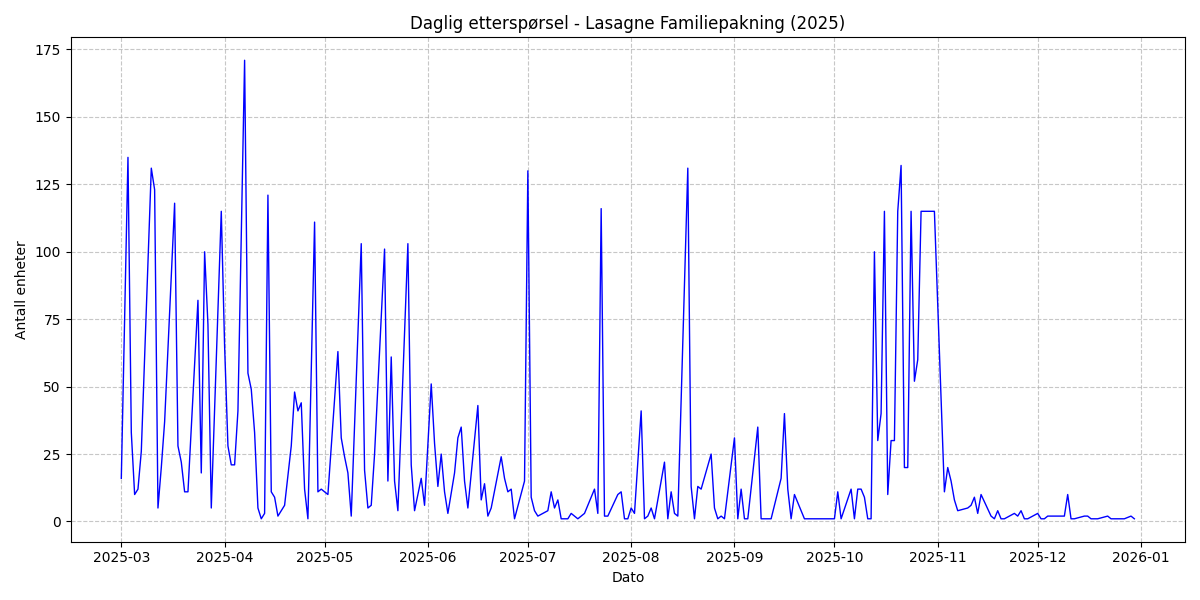
\includegraphics[keepaspectratio,alt={Figur 1: Historisk tidsserie for Lasagne Familiepakning}]{figurer/fig1_tidsserie.png}}
\caption{Figur 1: Historisk tidsserie for Lasagne Familiepakning}
\end{figure}

\emph{Figur 1: Historisk tidsserie (mars 2025 -- februar 2026) som viser
variasjon i utlevert volum. De to største toppene inntreffer i uken før
Crazy Days høst (uke 44/2025) og i uken etter oppstart av Crazy Days
vinter (uke 6/2026).}

Nivået ligger stabilt lavt i normalperioder, men brytes av kortsiktige
og kraftige topper rundt kampanjeperiodene. Det er ingen tydelig
langsiktig trend, men en klar sesongvariasjon knyttet til ukedager.
Dette utdypes i Figur 2.

\begin{figure}
\centering
\pandocbounded{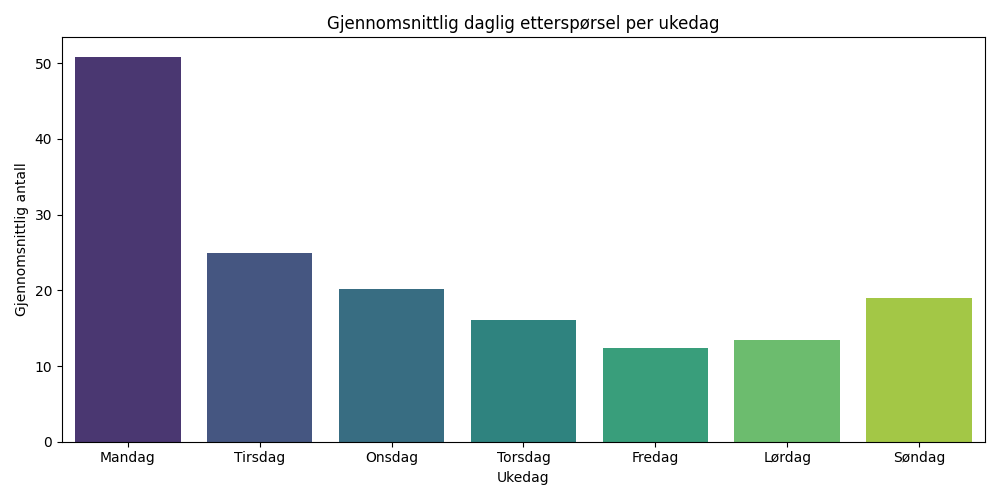
\includegraphics[keepaspectratio,alt={Figur 2: Gjennomsnittlig daglig utlevert volum per virkedag}]{figurer/fig2_ukedag.png}}
\caption{Figur 2: Gjennomsnittlig daglig utlevert volum per virkedag}
\end{figure}

\emph{Figur 2: Gjennomsnittlig daglig utlevert volum per virkedag
(plukkdato, n = 52 per dag, mars 2025 -- februar 2026), som dokumenterer
den systematiske mandagseffekten på distribusjonssenteret.}

Mandager har det desidert høyeste gjennomsnittet (113,6 stk), etterfulgt
av tirsdag (97,3), onsdag (82,1), torsdag (67,4) og fredag (37,6). Den
fallende profilen gjennom uka skyldes at helgebestillinger akkumuleres
og ekspederes på mandag, slik at mandag i praksis rommer tre dagers
utleveringsbehov, mens fredagen er lavest fordi butikkene unngår
bestillinger de ikke rekker å motta før helgen. Denne systematiske
variasjonen er en kritisk innsikt som modellene i kap. 6 må kunne fange
opp.

\subsubsection{Bestillingsdato vs
plukkdato}\label{bestillingsdato-vs-plukkdato}

Det er viktig å skille mellom \textbf{bestillingsdato} (når butikken
oppretter ordren) og \textbf{plukkdato/utleveringsdato} (når varene
faktisk går ut fra distribusjonssenteret). Figur 2 viser plukkdato; det
er denne serien modellene predikerer fordi den bestemmer plukk- og
pakkekapasiteten ved distribusjonssenteret. Utleveringer skjer så å si
utelukkende på virkedager. Noen få lørdags- og søndagsutleveringer
forekommer gjennom året, typisk i tilknytning til høytider som påske, og
er derfor holdt utenfor figuren. Bestillinger registreres derimot hele
uka, også lørdag og søndag, og har et helt annet ukedagsmønster. Dette
synliggjøres i Figur 3.

\begin{figure}
\centering
\pandocbounded{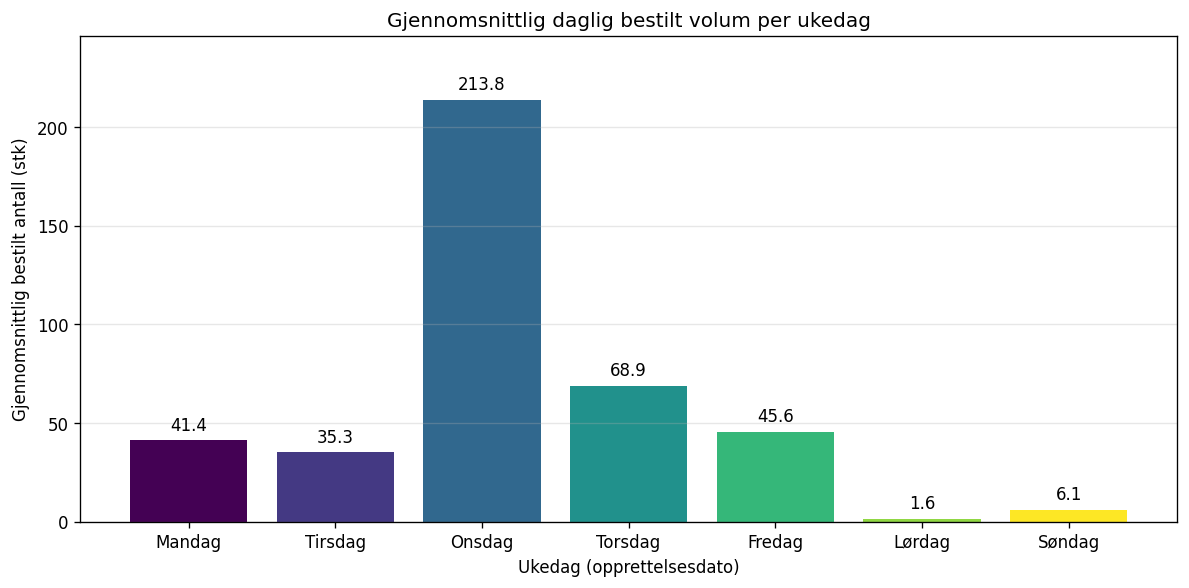
\includegraphics[keepaspectratio,alt={Figur 3: Gjennomsnittlig daglig bestilt volum per ukedag}]{figurer/fig3_bestilling_ukedag.png}}
\caption{Figur 3: Gjennomsnittlig daglig bestilt volum per ukedag}
\end{figure}

\emph{Figur 3: Gjennomsnittlig daglig bestilt volum per ukedag
(opprettelsesdato, alle 7 dager, mars 2025 -- februar 2026). Snitt
beregnet per kalenderdag i perioden, inkludert dager uten registrerte
bestillinger.}

Onsdag er den klart dominerende bestillingsdagen (213,8 stk), etterfulgt
av torsdag (68,9), fredag (45,6), mandag (41,4) og tirsdag (35,3).
Lørdag (1,6) og søndag (6,1) er marginale. Onsdagstoppen reflekterer at
butikkene legger inn hovedtyngden av ukens ordrer midt i uka, og at
disse plukkes på torsdag/fredag og delvis på mandag påfølgende uke.
Bestilling- og utleveringsprofilene er altså faseforskjøvet:
bestillingssignalet kommer onsdag, kapasitetsbehovet på
distribusjonssenteret inntreffer mandag. Totalt bestilt i perioden er 20
934 stk, mot 20 697 stk faktisk plukket og levert
(\texttt{Justert\ antall}, jf. datakildekontrollen i 4.3), et avvik på
1,1 \% av bestilt volum som skyldes justering mellom opprinnelig bestilt
og faktisk plukket antall.

\subsection{4.5 Kampanjemekanikk og
salgstopper}\label{kampanjemekanikk-og-salgstopper}

To Crazy Days-kampanjer er dokumentert av REMA i perioden: uke 45/2025
(3.--9. november) og uke 5/2026 (26. januar--1. februar). Figur 4 viser
ukentlig utlevert volum gjennom hele analyseperioden, med kampanje- og
hendelsesmarkeringer.

\begin{figure}
\centering
\pandocbounded{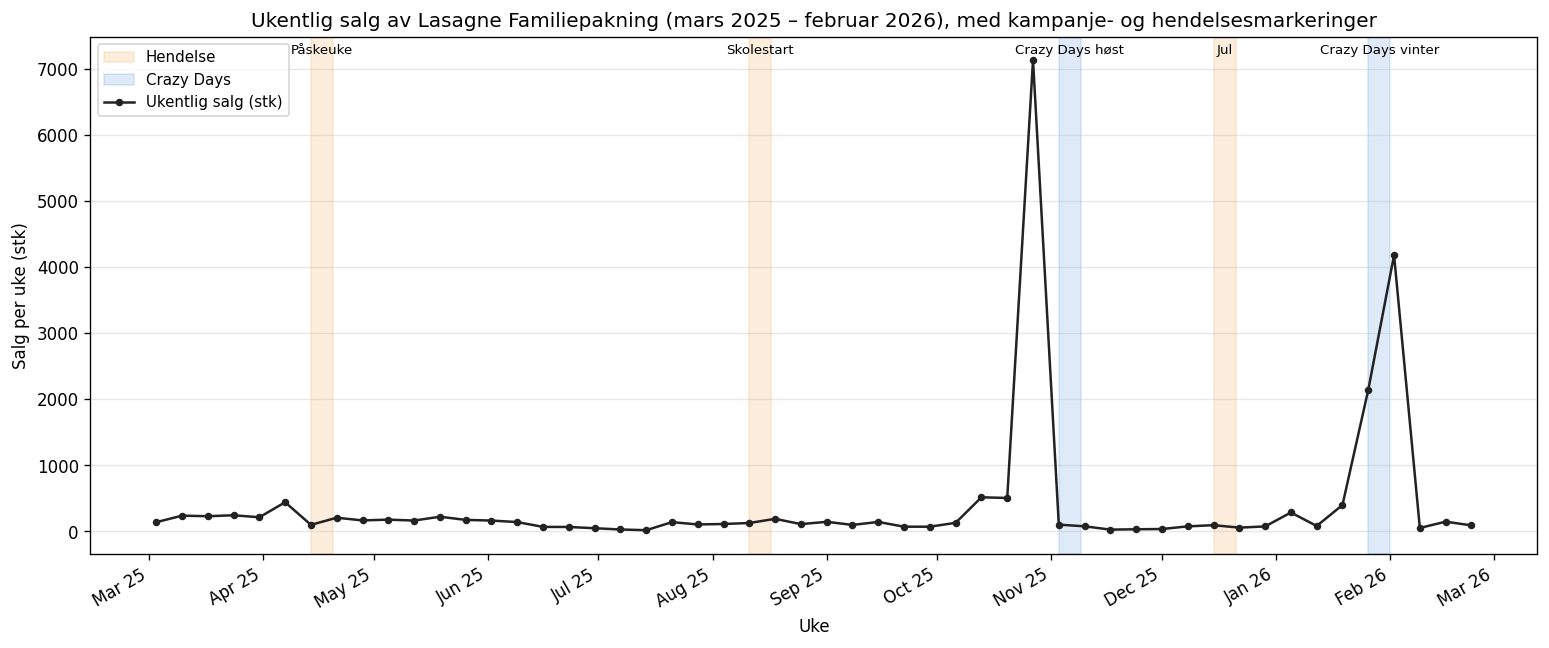
\includegraphics[keepaspectratio,alt={Figur 4: Ukentlig salg med kampanje- og hendelsesmarkeringer}]{figurer/fig4_kampanjeoversikt.png}}
\caption{Figur 4: Ukentlig salg med kampanje- og hendelsesmarkeringer}
\end{figure}

\emph{Figur 4: Ukentlig utlevert volum for Lasagne Familiepakning (mars
2025 -- februar 2026). Blå bokser markerer Crazy Days-kampanjer; oransje
bokser markerer hendelser (påske, skolestart, jul).}

Det mest karakteristiske mønsteret er at \textbf{salgstoppen inntreffer
i uken før selve kampanjen}, ikke under kampanjen. For Crazy Days høst
ligger uke 44 (27.--30. oktober) på 7 131 stk totalt, med dagsverdier 1
082--2 172 stk og maksimum onsdag 29. oktober. Selve kampanjeuken 45 har
bare 504 stk. For Crazy Days vinter er bildet todelt: kampanjeuken (uke
5) ligger på 2 140 stk, mens uken etter (uke 6, 2.--6. februar) topper
seg på 4 180 stk med dagsverdier opp mot 1 378 stk.

Dette reflekterer logistikken i distribusjonskjeden: butikkene legger
inn kampanjeordrer i forkant for å ha varer i butikk ved kampanjestart,
og distribusjonssenteret plukker og ekspederer disse ordrene noen dager
før kampanjen begynner. I praksis er det derfor \textbf{pre-campaign
stocking} som er driveren bak de største utleveringsvolumene, ikke
kampanjeuken i seg selv. For prognosemodellering innebærer dette at
kampanjeflagget må være aktivt i uken(e) før selve kampanjeperioden,
ikke bare under den (se kap. 6.3).

I motsetning til det man kunne forvente, viser dataene \textbf{ingen
julespike}. Dagsverdiene 22.--26. desember 2025 er 37, 18, 0, 0 og 0
stk, og uke 52 har totalt kun 55 stk. Dette skyldes trolig at
distribusjonssenteret stenger på helligdagene og at butikkene dekker
julehandelen gjennom ekstraordinære leveranser i tidligere uker. Heller
ikke påske (uke 16) eller skolestart (uke 33) gir noen tydelig salgstopp
i data, selv om de er merket i REMAs hendelseskalender.

De observerte toppene reflekterer \textbf{reell, utlevert etterspørsel},
og inneholder ikke noe kapasitetstak (``Censored Demand''). Ifølge PK
hos REMA har distribusjonslageret aldri vært utsolgt i perioden (se
dokumentasjon i Vedlegg A8), og det er ingen ``flate platåer'' i
datasettet som indikerer logistisk avskjæring. Volumet under Crazy Days
styres i praksis av kombinasjonen butikkbestillinger (via AOF/RELEX) og
sentralt allokert kampanjevolum, og kan derfor variere kraftig fra én
kampanje til en annen.

\subsection{4.6 Konsekvenser og behov for
modeller}\label{konsekvenser-og-behov-for-modeller}

Mangelen på presise prognoser har direkte operative konsekvenser for
REMA 1000: * \textbf{Stock-outs:} Ved underestimering risikerer man
tomme hyller og tapt salg. * \textbf{Lagerbinding:} Ved overestimering
øker lagerkostnadene og kapitalbindingen på distribusjonssenteret. *
\textbf{Uforutsigbarhet:} Brå topper skaper press på transportkapasitet
og bemanning.

Siden butikkenes ordrer godkjennes med \textasciitilde100 \% aksept for
tørrvarer, er prognosens kvalitet nærmest direkte bestemmende for
bestilt volum. En modell som både håndterer den stabile
virkedagssyklusen og de kraftige kampanje-/høytidstoppene, er derfor en
konkret driver for operasjonell effektivitet. Dette danner grunnlaget
for metodevalget (kap. 5) og modellvalget (kap. 6).

\section{5. Metode og data}\label{metode-og-data}

Dette kapittelet redegjør for studiens metodiske tilnærming,
datagrunnlaget og den trinnvise prosessen som er benyttet for å besvare
problemstillingen. Formålet er å sikre at analysen er transparent og
etterprøvbar.

\subsection{5.1 Metodevalg og
forskningsstruktur}\label{metodevalg-og-forskningsstruktur}

Studien benytter et \textbf{kvantitativt forskningsdesign} basert på en
case-studie av REMA 1000 Distribusjon Trondheim. Valget av kvantitativ
metode er begrunnet i behovet for å analysere store mengder historiske
transaksjonsdata for å identifisere mønstre og evaluere numerisk
nøyaktighet i prognoser.

Arbeidet er strukturert som en lineær prosess der målet er å
identifisere den mest robuste modellen for å håndtere ``Lumpy Demand''.
Ved å kombinere klassisk statistikk (SARIMA; Box \& Jenkins, 1976) med
maskinlæring (Random Forest; Breiman, 2001), oppnår vi en metodisk
triangulering som øker studiens faglige tyngde og gir et mer nyansert
bilde av prediksjonsevnen.

\subsection{5.2 Den analytiske
prosessen}\label{den-analytiske-prosessen}

Analysen er gjennomført i fire hovedfaser ved bruk av Python 3 og
bibliotekene Pandas (McKinney, 2010), Statsmodels (Seabold \& Perktold,
2010) og Scikit-learn (Pedregosa et al., 2011). Dette delkapittelet gir
en oversikt over flyten; tekniske detaljer er beskrevet der teknikkene
faktisk anvendes.

\begin{enumerate}
\def\labelenumi{\arabic{enumi}.}
\tightlist
\item
  \textbf{Dataklargjøring (vask):} RELEX-eksporten pivoteres fra bredt
  til langt format og filtreres til virkedager; ERP-uttrekket brukes som
  uavhengig kryssjekk (kap. 4.3).
\item
  \textbf{Modellering og estimering:} Åtte modeller trenes på
  treningssettet. Modellutvalg og feature engineering er beskrevet i
  kap. 6, og parametersøk og kryssvalidert tuning i kap. 7.2.
\item
  \textbf{Validering:} Modellene testes på det uavhengige testsettet, og
  residualstrukturen vurderes med formelle tester. Stasjonaritetstest av
  treningsserien er beskrevet i kap. 7.1, og residualdiagnostikk i kap.
  7.4.
\item
  \textbf{Evaluering:} Modellene sammenlignes med fem komplementære
  feilmål, segmentert på normale dager og toppdager.
  Evalueringsprotokoll og feilmål er beskrevet i kap. 5.7 og 5.8.
\end{enumerate}

\subsection{5.3 Datagrunnlag, struktur og
lagerstatus}\label{datagrunnlag-struktur-og-lagerstatus}

Primærdataene er daglig salg hentet fra REMA 1000s prognoseverktøy
\textbf{RELEX}. For å bekrefte at salgsdataene er et pålitelig mål for
etterspørsel, har vi i tillegg gjennomgått lagerstatus for hele
analyseperioden via et skjermbilde fra RELEX-grensesnittet (Vedlegg A8).
Oversikten viser at lagernivået aldri når null, og at
distribusjonssenteret aldri har vært utsolgt på Lasagne Familiepakning i
analyseperioden. Dette validerer antagelsen om at observerte salgstall
reflekterer faktisk utlevert etterspørsel, ikke en kapasitetsbegrenset
restetterspørsel.

\begin{itemize}
\tightlist
\item
  \textbf{Kilde:} RELEX Solutions-eksport (daglig aggregert) og REMA
  1000 ERP-systemer (lagerstatus).
\item
  \textbf{Periode:} 1. mars 2025 -- 28. februar 2026 (365 kalenderdager,
  260 virkedager etter filtrering).
\item
  \textbf{Variabel:} Daglig utlevert volum i antall enheter (stk).
\end{itemize}

\subsection{5.4 Datakvalitet, antagelser og
begrensninger}\label{datakvalitet-antagelser-og-begrensninger}

Dataene anses som høyt reliable. De representerer faktiske fysiske
bevegelser ved distribusjonssenteret, og RELEX-eksporten krysstemmer
innen 0,6 \% mot et uavhengig ERP-uttrekk på transaksjonsnivå (kap.
4.3).

\textbf{Viktige antagelser og metodiske grep:} *
\textbf{Virkedagsfiltrering:} Helgedager (lør/søn) ekskluderes. Dette
gir en ren 5-dagers syklus som er kompatibel med SARIMA med periode s=5
og med virkedagsbaserte lag-features. Tapet på 100 stk (12 helgdager med
observert salg \textgreater{} 0) utgjør 0,5 \% av totalen og endrer ikke
konklusjonene. * \textbf{Etterspørsel = utlevert volum:} Fordi lageret
aldri var utsolgt, antar vi at utlevert volum reflekterer den faktiske
etterspørselen fra butikkene. Det er ingen ``Censored Demand''-effekter
i datagrunnlaget. * \textbf{Kampanjeeffekter:} Kampanjekalender med to
Crazy Days-perioder (uke 45/2025, uke 5/2026) og tre hendelser (påske,
skolestart, jul) er lagret i \texttt{004\ data/kampanjekalender.csv} og
leses inn ved modellkjøring. * \textbf{Oppdaget datafeil korrigert:} Et
tidligere vaskeskript (\texttt{vask\_data.py}) produserte et feil
aggregert datasett (sum 6 201 stk i stedet for de faktiske 20 701 stk i
RELEX-virkedagsserien, jf. 4.3). Feilen ble oppdaget ved kryssjekk mot
RELEX-eksport og er rettet. Detaljer er dokumentert i kap. 9.1.

\subsection{5.5 Etiske hensyn og
konfidensialitet}\label{etiske-hensyn-og-konfidensialitet}

Studien er gjennomført under taushetserklæring signert med REMA 1000, og
datagrunnlaget består utelukkende av aggregert salgs- og lagerstatistikk
for ett produkt ved ett distribusjonssenter. Dataene inneholder ingen
kunde-, ansatt- eller persondata, slik at personvernforordningen (GDPR)
ikke er direkte berørt. Eksporter fra RELEX og ERP-systemet anses
likevel som forretningssensitive fordi de avdekker intern operasjonell
aktivitet, og er lagret lokalt på prosjektgruppens enheter. Rådata
distribueres ikke utenfor prosjektet; deling med tredjepart skjer kun
gjennom rapportens eksplisitt rapporterte aggregater (statistikker,
modellresultater, figurer) og avidentifiserte mellomprodukter som
\texttt{004\ data/vasket\_salg\_daglig.csv}. Bedriftsspesifikke detaljer
som omfanget eller tidspunktet for konkrete kampanjer fremstilles bare i
den grad det er nødvendig for analysens etterprøvbarhet.

\subsection{5.6 Oppdeling av data (trening og
test)}\label{oppdeling-av-data-trening-og-test}

For å simulere en reell prognosesituasjon og sikre at vi måler
modellenes generaliseringsevne (out-of-sample), er datasettet delt inn
slik: * \textbf{Treningssett:} 1. mars 2025 -- 31. desember 2025, 218
virkedager. SARIMA og baseliner (Seasonal Naïve, Holt-Winters) trenes på
hele settet. For ML-modeller med lag- og rolling-features (RF, GBM)
reduseres effektivt treningssett til 208 dager fordi de 10 første dagene
mangler komplette features. * \textbf{Testsett:} 1. januar 2026 -- 28.
februar 2026 (42 virkedager).

Splitten tilsvarer \textasciitilde83/17 \% av de tilgjengelige
observasjonene. Testperioden inneholder Crazy Days uke 5/2026, noe som
gir anledning til å evaluere modellenes evne til å prediktere
kampanjeeffekter som ikke overlapper treningssettet fullt ut.

\subsection{5.7 Evalueringsprotokoll}\label{evalueringsprotokoll}

Evalueringsprotokollen følger en blandet logikk som er viktig å være
transparent om, fordi den får direkte konsekvenser for hvordan
resultatene i kap. 8 skal tolkes. SARIMA og Holt-Winters trenes én gang
på treningssettet (1. mars -- 31. desember 2025) og produserer deretter
en sammenhengende \textbf{multi-step-prognose} for hele testperioden på
42 virkedager. Modellene refittes ikke underveis, og ingen testdata
flyter inn i parameterestimatet. Seasonal Naïve, Random Forest, Random
Forest uten lag\_1 og Gradient Boosting bruker derimot lag-features som
er bygd én gang på den fullstendige tidsserien. Dette betyr at modellen
for hver testdag har tilgang til faktiske observerte verdier fra
foregående dager via lag\_1, lag\_5, lag\_10 og rolling\_mean\_5. I
praksis gir disse fire modellene altså en \textbf{én-steg-frem-prognose}
med ekte observert lag, mens SARIMA og Holt-Winters gir en
multi-step-prognose uten oppdatering av observasjoner.

Begrunnelsen for å bruke faktiske lag-verdier i ML-modellene er at dette
reflekterer den operasjonelle virkeligheten i REMAs
dag-for-dag-bestillingsprosess (kap. 4.1): når dagens prognose lages, er
gårsdagens utleverte volum allerede observert. Praksisen er i tråd med
Hyndman og Athanasopoulos (2021) sin anbefaling om å la
prognoseprotokollen speile beslutningssituasjonen. Konsekvensen er at
modellene ikke konkurrerer på helt like vilkår: SARIMA og Holt-Winters
må predikere 42 dager fram uten å se observasjoner underveis, mens
Seasonal Naïve, Random Forest, Random Forest uten lag\_1 og Gradient
Boosting har tilgang til faktiske observerte verdier fra foregående
dager via lag- og rolling-features. Asymmetrien er sentral for
tolkningen av resultatene i kap. 8 og kan påvirke hvilken modell som
fremstår som best i de aggregerte feilmålene. En streng sammenligning
mellom modellfamilier krever derfor at protokollforskjellen leses sammen
med tabellene, og hybridmodellene i kap. 6.2 er konstruert nettopp for å
utnytte den komplementære styrken hver familie viser under sin egen
protokoll.

\subsection{5.8 Evalueringsmål}\label{evalueringsmuxe5l}

Vi rapporterer fem komplementære mål: * \textbf{MAE} (Mean Absolute
Error): gjennomsnittlig absoluttfeil i stk. Enkel å kommunisere, og gir
ikke skjeve utslag ved lave verdier. * \textbf{MAPE} (Mean Absolute
Percentage Error): rapportert av tradisjon, men tolkes med forbehold.
Dager med svært lavt volum gjør MAPE ustabil. * \textbf{sMAPE}
(symmetric MAPE): skalainvariant og robust mot lave nevnere, verdier i
{[}0, 200 \%{]}. * \textbf{WAPE} (Weighted Absolute Percentage Error):
total absoluttfeil vektet med totalt volum, egnet for volumprioritert
logistikkbeslutning. * \textbf{Bias}: gjennomsnittlig signert feil.
Positiv verdi = overestimering; negativ = underestimering. Sentralt mål
for sikkerhetslagerdimensjonering (Seiringer et al., 2022).

\subsection{5.9 Oppsummering --- tekniske
nøkkeltall}\label{oppsummering-tekniske-nuxf8kkeltall}

Tabell 2 oppsummerer beskrivende statistikk for daglig utlevert volum
(stk) i trenings- og testsettet. Tallene gir leseren en kompakt
referanse for hva modellene faktisk skal predikere, og hvor stor
variasjonen er mellom segmentene.

{\def\LTcaptype{none} % do not increment counter
\begin{longtable}[]{@{}lrr@{}}
\toprule\noalign{}
Statistikk & Treningssett (218 dager) & Testsett (42 dager) \\
\midrule\noalign{}
\endhead
\bottomrule\noalign{}
\endlastfoot
Min & 0 & 0 \\
Maks & 2 172 & 1 378 \\
Gjennomsnitt & 61,1 & 175,6 \\
Median & 19,5 & 26,0 \\
Standardavvik & 239,3 & 320,9 \\
90. persentil & 70,6 & 508,8 \\
Toppdager (\textgreater P90 trening) & 22 & 15 \\
Sum & 13 327 & 7 374 \\
\end{longtable}
}

\emph{Tabell 2: Beskrivende statistikk for daglig utlevert volum (stk) i
trenings- og testsettet. Kilde:
\texttt{004\ data/vasket\_salg\_daglig.csv}.}

Testsettet inneholder Crazy Days uke 5/2026 og har derfor høyere
gjennomsnitt og maksverdi relativt til antall dager enn treningssettet.
Forskjellen i 90. persentil (70,6 vs 508,8 stk) illustrerer at
testperioden er kampanjedrevet og dermed et krevende, men relevant
scenario for å måle modellenes generaliseringsevne mot toppdager.

\section{6. Modellering}\label{modellering}

Dette kapittelet definerer og begrunner modellrammeverket. Modellvalget
er et resultat av en iterativ utvalgsprosess basert på
etterspørselsdataens struktur slik den er kartlagt i kap. 4: en sterk
virkedags-sesongvariasjon, kraftige kampanje- og høytidstopper, og en
treningsperiode på 218 virkedager (208 for maskinlæringsmodellene, etter
at de ti første dagene faller bort på grunn av lag-padding, jf. kap.
5.6).

\subsection{6.1 Arbeidsprosess og
modellutvalg}\label{arbeidsprosess-og-modellutvalg}

I den innledende fasen vurderte vi flere klasser av enklere
prognosemodeller før vi avgjorde det endelige rammeverket.
\textbf{Moving Average (MA)} ble testet i tre vindusstørrelser --- MA5,
MA10 og MA21, det vil si glidende gjennomsnitt over henholdsvis fem, ti
og 21 virkedager --- for å se om en ren utglattingsbasert tilnærming
kunne gi en akseptabel baseline. Modellen ble forkastet som
primærkandidat fordi den per konstruksjon utviser treghet ved brå
volumendringer og glatter ut nettopp de kampanjetoppene som er mest
kritiske for logistikkplanleggingen. \textbf{Holt-Winters} ble derimot
beholdt som klassisk baseline ved siden av Seasonal Naive: metoden er
enkel og rask å estimere, og den representerer den klassiske
eksponensielle utglattingsfamilien (Hyndman \& Athanasopoulos, 2021,
kap. 8) på en måte som komplementerer SARIMA uten å overlappe den.

Vi vurderte også å inkludere ren \textbf{ARMA(p,q)} uten sesongledd som
egen kandidat, gitt at ADF-testen i kap. 7.1 viser at den rå
virkedagsserien er stasjonær. ARMA er imidlertid et spesialtilfelle av
SARIMA-strukturen \((p,d,q)(P,D,Q)_s\): kombinasjonen \(d=0\), \(D=0\)
inngår i grid-søket beskrevet i kap. 7.2, slik at en ren ARMA-modell vil
bli valgt automatisk dersom AIC-kriteriet favoriserer den. Vi anså det
derfor som lite hensiktsmessig å føre opp ARMA som separat
kandidatmodell.

På den mer komplekse siden vurderte vi \textbf{Prophet} og
\textbf{LSTM-nevralnettverk}. Prophet ble vurdert som mindre nødvendig
gitt at SARIMA allerede tilbyr en robust statistisk struktur for sesong,
trend og eksogene regressorer, og at vi ønsket en parametrisert modell
vi kunne tolke direkte mot ACF/PACF-diagnostikken. LSTM ble forkastet på
prinsipielt grunnlag: dype rekurrente nett krever typisk fra noen tusen
til titusener av observasjoner for å oppveie for sin økte
modellkompleksitet, og er erfaringsmessig sjelden konkurransedyktige med
klassiske modeller på korte serier (Hyndman \& Athanasopoulos, 2021;
Makridakis et al., 2022). 218 treningsdager faller godt under den
terskelen, og en LSTM ville her risikert å overtilpasse til de få
kampanjetoppene i datasettet.

\subsection{6.2 Valgte modeller og deres utfyllende
roller}\label{valgte-modeller-og-deres-utfyllende-roller}

Åtte modeller er estimert for å dekke et bredt metodisk spenn fra enkle
baselines til hybride kombinasjoner. Tabell 3 oppsummerer modellene
langs deres viktigste karakteristika; den underliggende prosaen
forklarer hvorfor hver familie er representert.

De to \textbf{baselinene} etablerer en minimumsforventning som mer
komplekse modeller må slå for å rettferdiggjøre sin kompleksitet.
\textbf{Seasonal Naïve} setter prognosen for en dag lik faktisk volum
fra samme ukedag forrige uke (\(y_{t-5}\) på virkedagskalender) og
fanger ukedagssyklusen direkte uten estimerte parametre.
\textbf{Holt-Winters} med additiv trend og additiv sesongkomponent
(\(s=5\)) er en parametrisk eksponensiell utjevning som gir et
alternativ til SARIMA uten differensiering. Sammen illustrerer de hva en
helt enkel modell og en klassisk parametrisk modell hver for seg kan
oppnå.

Den \textbf{statistiske tidsseriemodellen} representeres av
\textbf{SARIMA} (\((p,d,q)(P,D,Q)_5\)) med eksogene regressorer for
kampanjeperioder (\texttt{is\_crazy\_days}, \texttt{is\_event}). SARIMA
er i Box \& Jenkins-tradisjonen (Box \& Jenkins, 1976) den naturlige
strukturelle modellen for serier med autoregressiv og
glidende-gjennomsnitt-dynamikk og en sesongkomponent. Parametervalget
skjer ved AIC-minimerende grid-search (kap. 7.2).

\textbf{Maskinlæringsfamilien} dekkes av tre varianter. \textbf{Random
Forest} (Breiman, 2001) trenes på et fullt feature-sett (variabelsett)
bestående av lag\_1, lag\_5, lag\_10, et 5-dagers glidende gjennomsnitt,
kalenderfeatures og kampanjeflagg, og er motivert av tre-basert
modellering sin evne til å fange ikke-lineære interaksjoner mellom
ukedag og kampanjeeffekter. \textbf{Random Forest uten lag\_1} er en
diagnostisk variant som fjerner forrige dags volum fra feature-vektoren;
hensikten er todelt. På den ene siden lar den oss undersøke hvor mye en
RF faktisk lærer utover en triviell ``i morgen = i dag''-strategi, og på
den andre siden viser senere analyse (kap. 8.3) at varianten i praksis
fungerer som operasjonell prognose for toppdager. Den er altså samtidig
et diagnostisk verktøy og en kandidatmodell. \textbf{Gradient Boosting}
(Friedman, 2001) bruker samme feature-vektor som Random Forest, men
sekvensiell tre-bygging i stedet for ensemble-snitt; hyperparametrene
velges ved 3-fold TimeSeriesSplit-kryssvalidering over 16 kombinasjoner
av læringsrate, treedybde, antall estimatorer og subsamplingsandel.

To \textbf{hybridmodeller} er konstruert for å teste om en kombinasjon
kan utnytte modellenes komplementære styrker. Den
\textbf{kampanje-baserte hybriden} ruter trafikken regelbasert: SARIMA
brukes på rutinedager, og RF uten lag\_1 brukes på dager markert i
kampanjekalenderen. Den \textbf{terskelbaserte hybriden} lar
prediksjonsapparatet selv bestemme rutingen --- SARIMA er default, men
dersom RF uten lag\_1 selv predikerer over 90.-persentilen i
treningssettet (terskel 70,6 stk), overtar RF-modellen for den dagen.
Den siste varianten har den praktiske fordelen at den ikke krever
eksplisitt kampanjeflagg ved prediksjonstidspunktet.

{\def\LTcaptype{none} % do not increment counter
\begin{longtable}[]{@{}
  >{\raggedright\arraybackslash}p{(\linewidth - 12\tabcolsep) * \real{0.1429}}
  >{\raggedright\arraybackslash}p{(\linewidth - 12\tabcolsep) * \real{0.1429}}
  >{\raggedright\arraybackslash}p{(\linewidth - 12\tabcolsep) * \real{0.1429}}
  >{\raggedright\arraybackslash}p{(\linewidth - 12\tabcolsep) * \real{0.1429}}
  >{\raggedright\arraybackslash}p{(\linewidth - 12\tabcolsep) * \real{0.1429}}
  >{\raggedright\arraybackslash}p{(\linewidth - 12\tabcolsep) * \real{0.1429}}
  >{\raggedright\arraybackslash}p{(\linewidth - 12\tabcolsep) * \real{0.1429}}@{}}
\toprule\noalign{}
\begin{minipage}[b]{\linewidth}\raggedright
\#
\end{minipage} & \begin{minipage}[b]{\linewidth}\raggedright
Modell
\end{minipage} & \begin{minipage}[b]{\linewidth}\raggedright
Familie
\end{minipage} & \begin{minipage}[b]{\linewidth}\raggedright
Sesongstruktur
\end{minipage} & \begin{minipage}[b]{\linewidth}\raggedright
Eksogene
\end{minipage} & \begin{minipage}[b]{\linewidth}\raggedright
Lag-features
\end{minipage} & \begin{minipage}[b]{\linewidth}\raggedright
Hyperparametersøk
\end{minipage} \\
\midrule\noalign{}
\endhead
\bottomrule\noalign{}
\endlastfoot
1 & Seasonal Naïve & Baseline & \(y_{t-5}\) & -- & -- & -- \\
2 & Holt-Winters & Baseline (ETS-familien) & additiv, \(s=5\) & -- & --
& -- \\
3 & SARIMA & Statistisk & \((P,D,Q)_5\) & \texttt{is\_crazy\_days},
\texttt{is\_event} & implisitt via AR-ledd & grid-search, 144
kombinasjoner (kap. 7.2) \\
4 & Random Forest & Maskinlæring & via lags og kalender & kampanjeflagg
& \(y_{t-1}\), \(y_{t-5}\), \(y_{t-10}\), rolling\_mean\_5 & -- (faste
defaults) \\
5 & RF uten lag\_1 & Maskinlæring (diagnostisk + operasjonell) & via
lags og kalender & kampanjeflagg & \(y_{t-5}\), \(y_{t-10}\),
rolling\_mean\_5 & -- \\
6 & Gradient Boosting & Maskinlæring & via lags og kalender &
kampanjeflagg & samme som RF & 3-fold TimeSeriesSplit, 16 kombinasjoner
(kap. 7.2) \\
7 & Hybrid (kampanje-router) & Hybrid & arvet fra delmodell &
regelbasert ruting & arvet & arvet \\
8 & Hybrid (terskelbasert) & Hybrid & arvet fra delmodell & -- & arvet &
terskel = 70,6 stk (P90 trening, 218 dager) \\
\end{longtable}
}

\emph{Tabell 3: Oversikt over de åtte estimerte modellene. Tabellen
tjener som referanse for kap. 7 (gjennomføring) og kap. 8 (resultater).}

\subsection{6.3 Datastrukturens påvirkning på
modellarkitekturen}\label{datastrukturens-puxe5virkning-puxe5-modellarkitekturen}

Tre strukturelle trekk i datagrunnlaget styrer modellarkitekturen, og
argumentene henger sammen som en sammenhengende begrunnelseskjede.

Den tydeligste strukturen er \textbf{virkedags-sesongvariasjonen}.
ACF-plott av treningsserien (kap. 7.1) viser sterke topper ved lag 5, 10
og 15, og dette mønsteret reflekteres direkte i modellvalgene: SARIMAs
sesongledd \((P,D,Q)_5\), Holt-Winters' \texttt{seasonal\_periods=5}, og
Random Forests bruk av \(y_{t-5}\) og \(y_{t-10}\) som lag-features
speiler alle den samme 5-dagers virkedagssyklusen. I tidligere
iterasjoner ble en 7-dagers syklus brukt, men den introduserte falske
helgemønstre fordi datagrunnlaget kun inneholder virkedager (jf. kap.
4.2 og kap. 5.4); overgangen til \(s=5\) er nærmere drøftet i kap. 9.1.

Et tilsvarende viktig trekk er \textbf{kampanje- og høytidstoppenes
ikke-lineære karakter}. Som kap. 4.3 dokumenterer, varierer dagsvolumet
på lasagne-pakningen med flere størrelsesordener mellom rutinedager og
kampanjedager, og effektene varierer på tvers av kampanjetyper.
Tre-baserte modeller fanger denne typen interaksjoner mellom ukedag,
lag-features og kampanjeflagg bedre enn lineære modeller, og dette er
den direkte motivasjonen for å inkludere Random Forest og Gradient
Boosting som primærmodeller for toppsegmentet.

Det tredje trekket er \textbf{stasjonariteten}. ADF-testen (kap. 7.1)
viser at både rå, første-ordens og sesongdifferensiert serie avviser
nullhypotesen om enhetsrot (alle p \textless{} 0,001), og den rå
virkedagsserien er altså stasjonær uten differensiering. SARIMAs
differensieringsledd (\(d\), \(D\)) er likevel ikke fastsatt på forhånd,
men inngår som søkeparametre i grid-søket beskrevet i kap. 7.2. Den
endelige modellen \((0,1,2)(0,1,1)_5\) er altså et resultat av
AIC-minimering, ikke et konservativt valg fra vår side. Hvorvidt
AIC-kriteriet straffer overdifferensiering tilstrekkelig på en allerede
stasjonær serie er en metodisk åpen problemstilling som drøftes i kap.
9.6.

\subsection{6.4 Modellspesifikasjon}\label{modellspesifikasjon}

For de \textbf{statistiske modellene} spesifiseres SARIMA som
\((p,d,q)(P,D,Q)_5\) med de eksogene regressorene
\texttt{is\_crazy\_days} og \texttt{is\_event}. Parametersettet velges
ved AIC-minimerende grid-search beskrevet i kap. 7.2. Holt-Winters
konfigureres med additiv trend og additiv sesong
(\texttt{trend=\textquotesingle{}add\textquotesingle{}},
\texttt{seasonal=\textquotesingle{}add\textquotesingle{}},
\texttt{seasonal\_periods=5}); initialisering av nivå- og
trendkomponenten skjer ved maksimum-likelihood-estimering på
treningssettet
(\texttt{initialization\_method=\textquotesingle{}estimated\textquotesingle{}}).

For \textbf{maskinlæringsmodellene} (Random Forest, Random Forest uten
lag\_1, Gradient Boosting) deles en felles feature-vektor med ett
unntak. Vektoren inneholder lag-features (\(y_{t-1}\), \(y_{t-5}\),
\(y_{t-10}\)), et 5-dagers glidende gjennomsnitt
(\texttt{rolling\_mean\_5}), kalenderfeatures (\texttt{is\_monday},
\texttt{month}, \texttt{week\_of\_month},
\texttt{days\_since\_last\_order}), ukedag-dummier og kampanjeflagg.
Random Forest uten lag\_1 mottar samme vektor minus \(y_{t-1}\).
Gradient Boosting deler vektor med Random Forest, men hyperparametrene
(læringsrate, treedybde, antall estimatorer og subsamplingsandel) tunes
ved kryssvalidert søk (kap. 7.2).

Variabeloversikten under sammenfatter symboler og features brukt i
modellene, slik at leseren kan navigere kap. 6--8 og vedlegg uten å bla
tilbake.

{\def\LTcaptype{none} % do not increment counter
\begin{longtable}[]{@{}
  >{\raggedright\arraybackslash}p{(\linewidth - 4\tabcolsep) * \real{0.3333}}
  >{\raggedright\arraybackslash}p{(\linewidth - 4\tabcolsep) * \real{0.3333}}
  >{\raggedright\arraybackslash}p{(\linewidth - 4\tabcolsep) * \real{0.3333}}@{}}
\toprule\noalign{}
\begin{minipage}[b]{\linewidth}\raggedright
Symbol/variabel
\end{minipage} & \begin{minipage}[b]{\linewidth}\raggedright
Beskrivelse
\end{minipage} & \begin{minipage}[b]{\linewidth}\raggedright
Rolle
\end{minipage} \\
\midrule\noalign{}
\endhead
\bottomrule\noalign{}
\endlastfoot
\(y_t\) & Daglig utlevert volum (stk) på virkedag \(t\) & Avhengig
variabel \\
\(y_{t-1}\) (\texttt{lag\_1}) & Foregående virkedags volum &
Lag-feature, ML \\
\(y_{t-5}\) (\texttt{lag\_5}) & Volum 5 virkedager tilbake (samme
ukedag) & Lag-feature, ML og SARIMA-sesong \\
\(y_{t-10}\) (\texttt{lag\_10}) & Volum 10 virkedager tilbake &
Lag-feature, ML \\
\texttt{rolling\_mean\_5} & 5-dagers glidende gjennomsnitt av \(y\) &
Glattingsvariabel, ML \\
\texttt{is\_monday} & Indikator: 1 hvis mandag, ellers 0 &
Kalenderfeature, ML \\
\texttt{month} & Kalendermåned (1--12) & Kalenderfeature, ML \\
\texttt{week\_of\_month} & Ukenummer i måneden (1--5) & Kalenderfeature,
ML \\
\texttt{days\_since\_last\_order} & Dager siden forrige observerte ordre
\textgreater{} 0 & Kalenderfeature, ML \\
\texttt{is\_crazy\_days} & Indikator: 1 hvis dag i Crazy Days-periode &
Eksogen regressor (SARIMA) / kampanjeflagg (ML) \\
\texttt{is\_event} & Indikator: 1 hvis dag i hendelse (påske, jul,
skolestart) & Eksogen regressor (SARIMA) / kampanjeflagg (ML) \\
\((p,d,q)(P,D,Q)_5\) & SARIMA-parametre --- ikke-sesong (p,d,q), sesong
(P,D,Q), periode 5 & SARIMA-spesifikasjon \\
70,6 stk & Toppdag-terskel (P90 av treningssettet, jf. Tabell 2) &
Segmenteringsterskel + hybrid (terskelbasert) \\
\end{longtable}
}

\emph{Variabeloversikt for modellene i kap. 6.}

Modellspesifikasjonene over definerer parametre og features, men
beskriver ikke selve evalueringsoppsettet. Den blandede protokollen, der
SARIMA og Holt-Winters opererer som multi-step-prognoser uten
oppdatering, mens ML-modellene opererer som én-steg-frem-prognoser med
faktisk observert lag, er forklart i kap. 5.7. Asymmetrien er sentral
for tolkningen av resultatene i kap. 8.

\subsection{6.5 Metodisk refleksjon}\label{metodisk-refleksjon}

Åtte modeller er valgt for å spenne over tre faglig distinkte
tilnærminger --- enkle baselines, en parametrisk statistisk modell og
ikke-parametriske maskinlæringsmodeller --- supplert med to
hybridvarianter. Hensikten er ikke utelukkende å maksimere
prognosepresisjon, men å gjennomføre en \textbf{metodisk triangulering}
som lar oss skille mellom feil som skyldes modellbegrensninger og feil
som skyldes egenskaper ved datagrunnlaget selv. M5-konkurransen
(Makridakis et al., 2022) viser nettopp at familie-diversitet og enkle
baselines er essensielle for å vurdere hva mer avanserte modeller
faktisk tilfører.

Trianguleringen tjener tre konkrete diagnostiske formål. Baselinene
definerer en minimumsforventning som de øvrige modellene må slå for å
rettferdiggjøre kompleksiteten. SARIMA gir et tolkbart, parametrisk
utgangspunkt der koeffisienter, AIC og residualstruktur kan inspiseres
direkte. Maskinlæringsvariantene utforsker ikke-lineære avhengigheter
som lineære modeller per definisjon ikke fanger, og den diagnostiske
RF-varianten uten lag\_1 gjør det mulig å vurdere hvor mye av Random
Forests prestasjon som faktisk skyldes læring av sesong- og
kampanjestruktur, og hvor mye som er en effekt av at \(y_{t-1}\) alene
er en sterk prediktor. Hybridmodellene tester den siste hypotesen --- at
en kombinasjon av komplementære modeller på rett segment kan slå hver
enkelt modell isolert. Til sammen gjør modellporteføljen analysen til
både et presisjonsestimat og et verktøy for å diagnostisere
etterspørselens natur ved REMA 1000.

\section{7. Analyse}\label{analyse}

Dette kapittelet dokumenterer den operative gjennomføringen av analysen:
stasjonaritetsvurdering, parameter-tuning, estimering og validering.

\subsection{7.1 Stasjonaritet og
ACF-vurdering}\label{stasjonaritet-og-acf-vurdering}

Før modellering ble treningsserien vurdert med hensyn til stasjonaritet
ved Augmented Dickey-Fuller-test (ADF; Dickey \& Fuller, 1979).
Resultatene (Tabell A1 i vedlegg) viser at både rå, første-ordens
differensiert og sesongdifferensiert (s=5) serie avviser nullhypotesen
om enhetsrot (p \textless{} 0,001). Serien er altså stasjonær allerede
uten differensiering.

Autokorrelasjonsfunksjonen (ACF) på den rå treningsserien er dominert av
en sterk autoregressiv struktur, med lag 1 = 0,79, lag 2 = 0,51 og lag 3
= 0,20, og verdier nær null fra lag 4 og utover. Dette mønsteret peker
på at dagens etterspørsel henger tett sammen med foregående dager, men
det er ingen sterk topp ved lag 5 i den rå serien som direkte avslører
en ukentlig syklus. Etter sesongdifferensiering (s=5) framtrer derimot
en betydelig negativ korrelasjon ved lag 5 (−0,51), noe som er det
klassiske mønsteret for en sesong-MA-komponent og dermed gir empirisk
støtte for et sesongledd i SARIMA. Selve valget av s=5 er først og
fremst en strukturell antagelse forankret i at distribusjonssenteret kun
ekspederer i virkedager (jf. kap. 4.2 og 5.4); ACF-mønsteret etter
sesongdifferensiering bekrefter at antagelsen er konsistent med dataene.

\subsection{7.2 Parametersøk og tuning}\label{parametersuxf8k-og-tuning}

SARIMA grid-search dekker 144 kombinasjoner av ordre
\((p,d,q) \in \{0,1,2\} \times \{0,1\} \times \{0,1,2\}\) og sesongordre
\((P,D,Q)_5 \in \{0,1\}^3\). AIC brukes som utvalgskriterium, og
modeller som ikke konvergerer kasseres. Beslutningen om å kassere
ikke-konvergerte modeller er prinsipiell: når MLE-optimeringen ikke
konvergerer, er parameterestimatene ikke pålitelige, og AIC-verdien blir
dermed ikke en meningsfull sammenligningsstørrelse på tvers av modeller.
Resultatene er tabellert i \texttt{004\ data/sarima\_diagnostikk.csv},
og topp 5 konvergerte kandidater er gjengitt i Vedlegg A2. Beste
konvergerte modell er \((0,1,2)(0,1,1)_5\) med AIC 2 510. Dette er en
forbedring på 48 AIC-poeng mot den opprinnelige \((1,1,1)(1,1,1)_7\)
(AIC 2 558), som var konfigurasjonen før virkedagskorrigeringen og
overgangen til 5-dagers sesongsyklus (jf. kap. 9.1). Flere
ikke-konvergerte kombinasjoner hadde numerisk lavere AIC, blant annet
\((1,0,2)(0,1,1)_5\) med AIC 2 481, men ble altså forkastet av
konvergensgrunner.

For Random Forest viser feature importance-analysen (variabelviktighet)
en utpreget dominans av \(y_{t-1}\) (lag\_1), som forklarer 84 \% av
variansen i full RF-variant. \texttt{rolling\_mean\_5} (7 \%),
\texttt{lag\_10} (2 \%) og \texttt{lag\_5} (2 \%) følger på de neste
plassene. Denne dominansen motiverer den diagnostiske RF-varianten uten
lag\_1, der \texttt{rolling\_mean\_5} (46 \%), \texttt{lag\_5} (25 \%)
og \texttt{lag\_10} (14 \%) overtar rollen som hoveddrivere. Den
fullstendige tabellen ligger i Vedlegg A4 og i
\texttt{004\ data/rf\_feature\_importance.csv}.

Gradient Boosting tunes ved 3-fold TimeSeriesSplit-kryssvalidering over
16 kombinasjoner av læringsrate, treedybde, antall estimatorer og
subsamplingsandel. Beste hyperparametere er
\texttt{learning\_rate=0,05}, \texttt{max\_depth=2},
\texttt{n\_estimators=100} og \texttt{subsample=1,0}. Tunet GBM gir
betydelig bedre MAE enn en utunet referanse med Sklearn-defaults
(\texttt{learning\_rate=0,1}, \texttt{max\_depth=3},
\texttt{n\_estimators=100}); reduksjonen er på rundt 30 \%, og
fullstendige cv-MAE-verdier per kombinasjon ligger i
\texttt{004\ data/gbm\_tuning.csv} og Vedlegg A3.

\subsection{7.3 Estimering og
segmentering}\label{estimering-og-segmentering}

Statistiske modeller (Seasonal Naive, Holt-Winters, SARIMA) trenes på
218 virkedager, og maskinlæringsmodellene (Random Forest, RF uten
lag\_1, Gradient Boosting) trenes på 208 virkedager etter at de ti
første dagene faller bort på grunn av lag-padding (jf. kap. 5.6). Alle
modeller evalueres på samme testsett på 42 virkedager (januar--februar
2026).

Gitt den ekstreme forskjellen mellom rutine- og kampanjedager evalueres
modellene segmentert basert på 90. persentilen fra hele treningssettet
(terskel 70,6 stk på 218 dager). Testsettets 42 virkedager fordeler seg
da i 27 normale dager (≤ 70,6 stk), som måler modellens presisjon i den
daglige stabile vareflyten, og 15 toppdager (\textgreater{} 70,6 stk),
som måler modellens evne til å håndtere kampanjer og ekstreme utslag.
Denne splittingen er avgjørende for å gi REMA 1000 et nyansert
beslutningsgrunnlag, fordi en modells styrke i ett segment kan
overskygge kritiske svakheter i et annet.

\subsection{7.4 Validering:
residualdiagnostikk}\label{validering-residualdiagnostikk}

For å validere at modellene har ekstrahert all systematisk informasjon
fra datasettet, evalueres residualene på to komplementære måter i tråd
med standard prognose-protokoll (Hyndman \& Athanasopoulos, 2021). Den
ene er en visuell ACF-inspeksjon, der residualer som ligger innenfor
konfidensintervallet indikerer hvit støy, og selve plottet presenteres
sammen med resultatene i kap. 8.3 (Figur 6). Den andre er Ljung-Box
Q-testen (Ljung \& Box, 1978) på ti etterslep (lags) i residualene, en
formell test der nullhypotesen er at residualene er uavhengige; en
p-verdi under 0,05 fører til at nullhypotesen forkastes og indikerer at
residualene fortsatt har mønster.

Som del av valideringsprotokollen inngår også systematisk bias per
segment, som avdekker i hvilken grad en modell konsekvent over- eller
underestimerer. Selve bias-tallene er presentert i kap. 8.3 sammen med
MAE og MAPE, mens den prinsipielle begrunnelsen for å inkludere bias som
validerings\-indikator hører hjemme her: bias-skjevhet har direkte
operasjonelle konsekvenser for sikkerhetslagerdimensjonering og
påliteligheten i transportplanlegging (Seiringer et al., 2022), og en
modell med lav MAE men stor systematisk bias er mindre operasjonelt
brukbar enn en modell med moderat MAE og balansert bias.

\section{8. Resultater}\label{resultater}

Dette kapittelet presenterer numeriske funn fra evalueringen av
prognosemodellene på testsettet (januar--februar 2026, 42 virkedager).
Resultatene er strukturert i fire deler: (8.1) sammenligning av Scenario
1 vs Scenario 2, (8.2) global modellytelse, (8.3) segmentert
resultatanalyse, og (8.4) residualdiagnostikk.

Før tabellene presenteres minner vi om protokollforskjellen redegjort
for i kap. 5.7: SARIMA og Holt-Winters opererer som multi-step-prognoser
uten oppdatering av observasjoner gjennom testperioden, mens Seasonal
Naïve, Random Forest, Random Forest uten lag\_1 og Gradient Boosting
opererer som én-steg-frem-prognoser med faktiske observerte lag-verdier.
Modellene konkurrerer derfor ikke på helt like vilkår, og rangering
basert på MAE alene må tolkes med dette forbeholdet.

Alle tall i resultattabellene bygger på
\texttt{scenario\_sammendrag.csv} fra \texttt{scenario\_analyse.py}, som
kjører Scenario 1 og 2 konsistent på samme datagrunnlag.
Ljung-Box-diagnostikken stammer fra en parallell kjøring i
\texttt{analyse\_hoved.py}; RF-variantene har identiske features i begge
skript (kun ulik rekkefølge), så de kvalitative konklusjonene om
residualstruktur er robuste.

\subsection{8.1 Sammenligning av Scenario 1 og Scenario
2}\label{sammenligning-av-scenario-1-og-scenario-2}

For å svare på problemstillingens delproblem 3, \emph{i hvilken grad
kampanjeaktivitet begrenser modellenes presisjon}, er alle modeller
kjørt i to scenarier: Scenario 1 (blind, kun historikk) og Scenario 2
(historikk pluss kampanje- og hendelsesindikatorer). Tabell 4
presenterer MAE for begge scenarier på tvers av seks modeller, globalt
over hele testsettet.

{\def\LTcaptype{none} % do not increment counter
\begin{longtable}[]{@{}
  >{\raggedright\arraybackslash}p{(\linewidth - 6\tabcolsep) * \real{0.2500}}
  >{\raggedleft\arraybackslash}p{(\linewidth - 6\tabcolsep) * \real{0.2500}}
  >{\raggedleft\arraybackslash}p{(\linewidth - 6\tabcolsep) * \real{0.2500}}
  >{\raggedleft\arraybackslash}p{(\linewidth - 6\tabcolsep) * \real{0.2500}}@{}}
\toprule\noalign{}
\begin{minipage}[b]{\linewidth}\raggedright
Modell
\end{minipage} & \begin{minipage}[b]{\linewidth}\raggedleft
Scenario 1 (blind)
\end{minipage} & \begin{minipage}[b]{\linewidth}\raggedleft
Scenario 2 (med kampanjeinfo)
\end{minipage} & \begin{minipage}[b]{\linewidth}\raggedleft
Endring
\end{minipage} \\
\midrule\noalign{}
\endhead
\bottomrule\noalign{}
\endlastfoot
Seasonal Naïve & 227,12 & 227,12 & 0,0 \% \\
Holt-Winters & 198,71 & 198,71 & 0,0 \% \\
SARIMA & 174,02 & \textbf{173,30} & −0,4 \% \\
Random Forest & 183,48 & 192,09 & +4,7 \% \\
RF uten lag\_1 & 178,99 & \textbf{169,11} & −5,5 \% \\
Gradient Boosting & 268,23 & 294,28 & +9,7 \% \\
\end{longtable}
}

\emph{Tabell 4: MAE (stk) på testsettet per scenario og modell}

Scenario 2 gir kun marginal global forbedring på SARIMA, som reduseres
med under 1 stk per dag (174,0 → 173,3 stk, −0,4 \%). RF uten lag\_1
forbedres mer markant (179,0 → 169,1 stk, −5,5 \%, drøyt 9 stk per dag),
mens Random Forest og GBM får dårligere globalytelse med kampanjeinfo.
Den segmenterte analysen (kap. 8.3) viser at dette skyldes hvordan
modellene fordeler forbedringer mellom normale dager og toppdager. Figur
5 illustrerer dette ved å vise faktisk etterspørsel (sort) sammen med RF
Scenario 1 (rødt), RF uten lag\_1 Scenario 2 (oransje) og Hybrid
terskelbasert Scenario 2 (grønn) over testperioden.

\begin{figure}
\centering
\pandocbounded{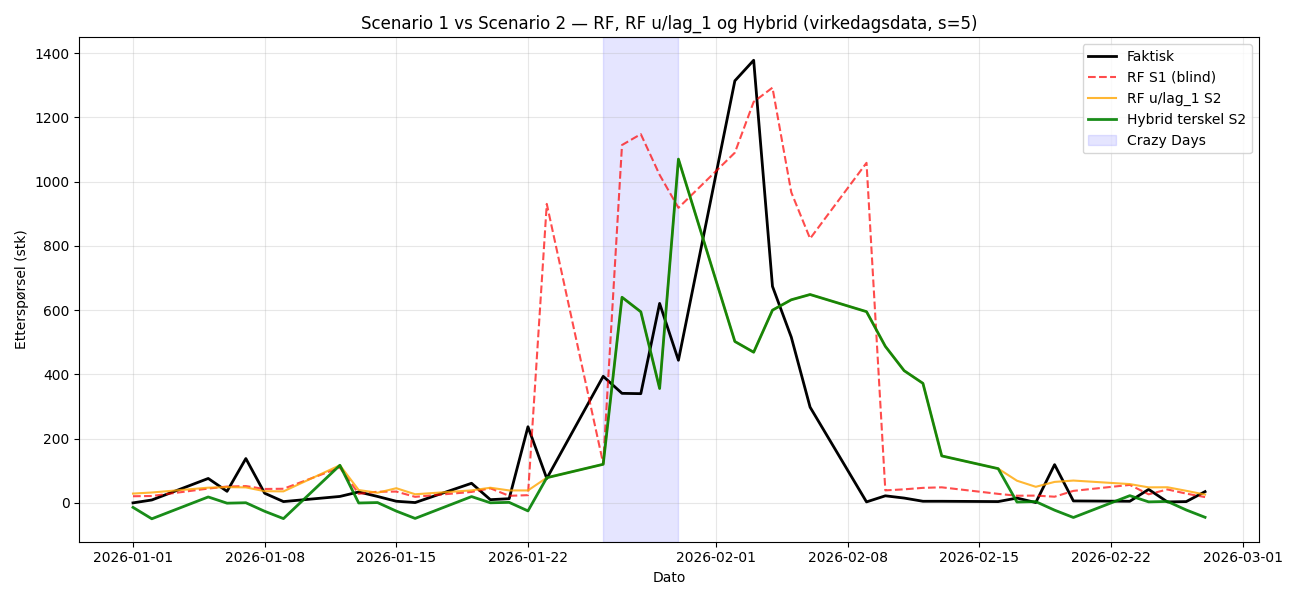
\includegraphics[keepaspectratio,alt={Figur 5: Scenario 1 vs Scenario 2 --- modellsammenligning}]{figurer/fig_scenario_sammenligning.png}}
\caption{Figur 5: Scenario 1 vs Scenario 2 --- modellsammenligning}
\end{figure}

\emph{Figur 5: Faktisk etterspørsel (sort) sammenlignet med RF Scenario
1 (rødt, blind), RF uten lag\_1 Scenario 2 (oransje) og Hybrid
terskelbasert Scenario 2 (grønn) over testperioden.}

\subsection{8.2 Global modellytelse}\label{global-modellytelse}

Tabell 5 sammenfatter den globale ytelsen (hele testsettet, 42
virkedager) for åtte modeller i Scenario 2, med fem feilmål.
Hybridmodellene er kun definert i Scenario 2 og kombinerer styrker fra
to enkelt\-modeller: Hybrid (kampanje) bruker SARIMA på dager uten
kampanje\-indikator og RF uten lag\_1 på kampanjedager, mens Hybrid
(terskel) velger SARIMA på normale dager (≤ 70,6 stk) og RF uten lag\_1
på toppdager (\textgreater{} 70,6 stk) basert på P90-terskelen fra
treningssettet (definert i detalj i kap. 9.4).

{\def\LTcaptype{none} % do not increment counter
\begin{longtable}[]{@{}lrrrrr@{}}
\toprule\noalign{}
Modell & MAE & MAPE & sMAPE & WAPE & Bias \\
\midrule\noalign{}
\endhead
\bottomrule\noalign{}
\endlastfoot
Seasonal Naive & 227,1 & 1 913 \% & 122 \% & 129 \% & −0,6 \\
Holt-Winters & 198,7 & 477 \% & 182 \% & 113 \% & −198,6 \\
SARIMA (grid) & 173,3 & 369 \% & 164 \% & 99 \% & −170,5 \\
Random Forest & 192,1 & 1 214 \% & 106 \% & 109 \% & +135,5 \\
\textbf{RF uten lag\_1} & \textbf{169,1} & 1 308 \% & 108 \% &
\textbf{96 \%} & +38,9 \\
Gradient Boosting & 294,3 & 1 629 \% & 107 \% & 168 \% & +253,6 \\
Hybrid (kampanje) & 177,7 & 371 \% & 159 \% & 101 \% & −118,7 \\
\textbf{Hybrid (terskel)} & 175,9 & 1 212 \% & 145 \% & 100 \% &
\textbf{+6,6} \\
\end{longtable}
}

\emph{Tabell 5: Global evaluering --- Scenario 2 (alle testdager).
MAPE-verdier er gjennomgående svært høye fordi små nevnere på
lavvolum-dager forsterker prosentfeilen; sMAPE og WAPE er mer robuste
tolkningsmål for denne typen serier (Hyndman \& Koehler, 2006).}

MAPE-verdiene er gjennomgående svært høye og skyldes dager med lavt
faktisk volum (små nevnere). sMAPE og WAPE gir mer tolkbare tall. RF
uten lag\_1 har lavest globale MAE (169,1) og WAPE (96 \%), og
terskelbasert hybrid har bias nær null (+6,6 stk).

\subsection{8.3 Segmentert
resultatanalyse}\label{segmentert-resultatanalyse}

Den segmenterte analysen separerer normale dager (≤ 70,6 stk) fra
toppdager (\textgreater{} 70,6 stk). Terskelen er 90.-persentilen av
treningssettet (218 virkedager), jf. kap. 7.3. Tabell 6 viser segmentert
MAE og Bias for de seks best presterende modellene under Scenario 2.

{\def\LTcaptype{none} % do not increment counter
\begin{longtable}[]{@{}llrr@{}}
\toprule\noalign{}
Segment & Modell & MAE & Bias \\
\midrule\noalign{}
\endhead
\bottomrule\noalign{}
\endlastfoot
\textbf{Normale dager} (n=27) & Seasonal Naive & 172,2 & +161,6 \\
& Holt-Winters & 38,5 & −38,2 \\
& \textbf{SARIMA} & \textbf{29,4} & \textbf{−25,1} \\
& Random Forest & 64,0 & +59,1 \\
& RF uten lag\_1 & 101,8 & +99,5 \\
& Hybrid (terskel) & 104,0 & +57,8 \\
\textbf{Toppdager} (n=15) & Seasonal Naive & 326,0 & −292,5 \\
& Holt-Winters & 487,2 & −487,2 \\
& SARIMA & 432,3 & −432,3 \\
& Random Forest & 422,6 & +273,0 \\
& \textbf{RF uten lag\_1} & \textbf{290,2} & \textbf{−70,3} \\
& Hybrid (terskel) & 305,5 & −85,5 \\
\end{longtable}
}

\emph{Tabell 6: Segmentert evaluering --- MAE og Bias per segment,
Scenario 2}

For å vise SARIMAs ulike respons på kampanjeinformasjon i de to
segmentene, sammenligner Tabell 6b modellen på tvers av Scenario 1 og
Scenario 2.

{\def\LTcaptype{none} % do not increment counter
\begin{longtable}[]{@{}lrrr@{}}
\toprule\noalign{}
Segment & Scenario 1 MAE & Scenario 2 MAE & Endring \\
\midrule\noalign{}
\endhead
\bottomrule\noalign{}
\endlastfoot
Normale dager (n=27) & 46,0 & \textbf{29,4} & −36 \% \\
Toppdager (n=15) & 404,5 & 432,3 & +7 \% \\
\end{longtable}
}

\emph{Tabell 6b: SARIMA segmentert MAE --- Scenario 1 vs Scenario 2}

Analysen avdekker en klart segmentert modellvinner-struktur. På normale
dager er SARIMA best (MAE 29,4); kampanjeinformasjon reduserer feilen
fra 46,0 (Scenario 1) til 29,4 (Scenario 2), en forbedring på 36 \%,
mens samme informasjon gir en svak forverring på toppdager (+7 \%). På
toppdager er RF uten lag\_1 best (MAE 290,2), tett fulgt av Hybrid
(terskel) (305,5), som har lavere absolutt bias.

Holt-Winters, full Random Forest og SARIMA har alle store bias på
toppdager (henholdsvis −487, +273 og −432), mens hybriden (terskel) har
\textbar Bias\textbar{} på 85 stk. Operasjonelle implikasjoner av disse
bias-forskjellene drøftes i kap. 9.4.

En observasjon som peker fram mot diskusjonen: både Holt-Winters og
SARIMA har \textbar Bias\textbar{} = MAE på toppdager (487 og 432). Når
Bias og MAE er like i absoluttverdi, må alle residualer ha samme
fortegn, det vil si at samtlige 15 toppdager undervurderes systematisk.
Mekanismen bak dette mønsteret diskuteres i kap. 9.3.

\subsection{8.4 Residualdiagnostikk og
modellvaliditet}\label{residualdiagnostikk-og-modellvaliditet}

For å teste om modellene har ekstrahert all systematisk informasjon, ble
Ljung-Box Q-test (10 etterslep / lags, jf. kap. 7.4) og ACF-plott
evaluert (Figur 6).

{\def\LTcaptype{none} % do not increment counter
\begin{longtable}[]{@{}lrrl@{}}
\toprule\noalign{}
Modell & Q-statistikk & p-verdi & Avviser H0 (autokorrelasjon)? \\
\midrule\noalign{}
\endhead
\bottomrule\noalign{}
\endlastfoot
Seasonal Naive & 63,4 & \textless{} 0,001 & Ja (mønster) \\
Holt-Winters & 68,0 & \textless{} 0,001 & Ja (mønster) \\
SARIMA (grid) & 53,6 & \textless{} 0,001 & Ja (mønster) \\
Random Forest & 13,5 & 0,195 & Nei (hvit støy) \\
RF uten lag\_1 & 12,8 & 0,236 & Nei (hvit støy) \\
Gradient Boosting & 30,0 & \textless{} 0,001 & Ja (mønster) \\
Hybrid (kampanje) & 12,9 & 0,231 & Nei (hvit støy) \\
Hybrid (terskel) & 13,0 & 0,223 & Nei (hvit støy) \\
\end{longtable}
}

\emph{Tabell 7: Ljung-Box Q-test på testresidualer (10 etterslep,
Scenario 2)}

\begin{figure}
\centering
\pandocbounded{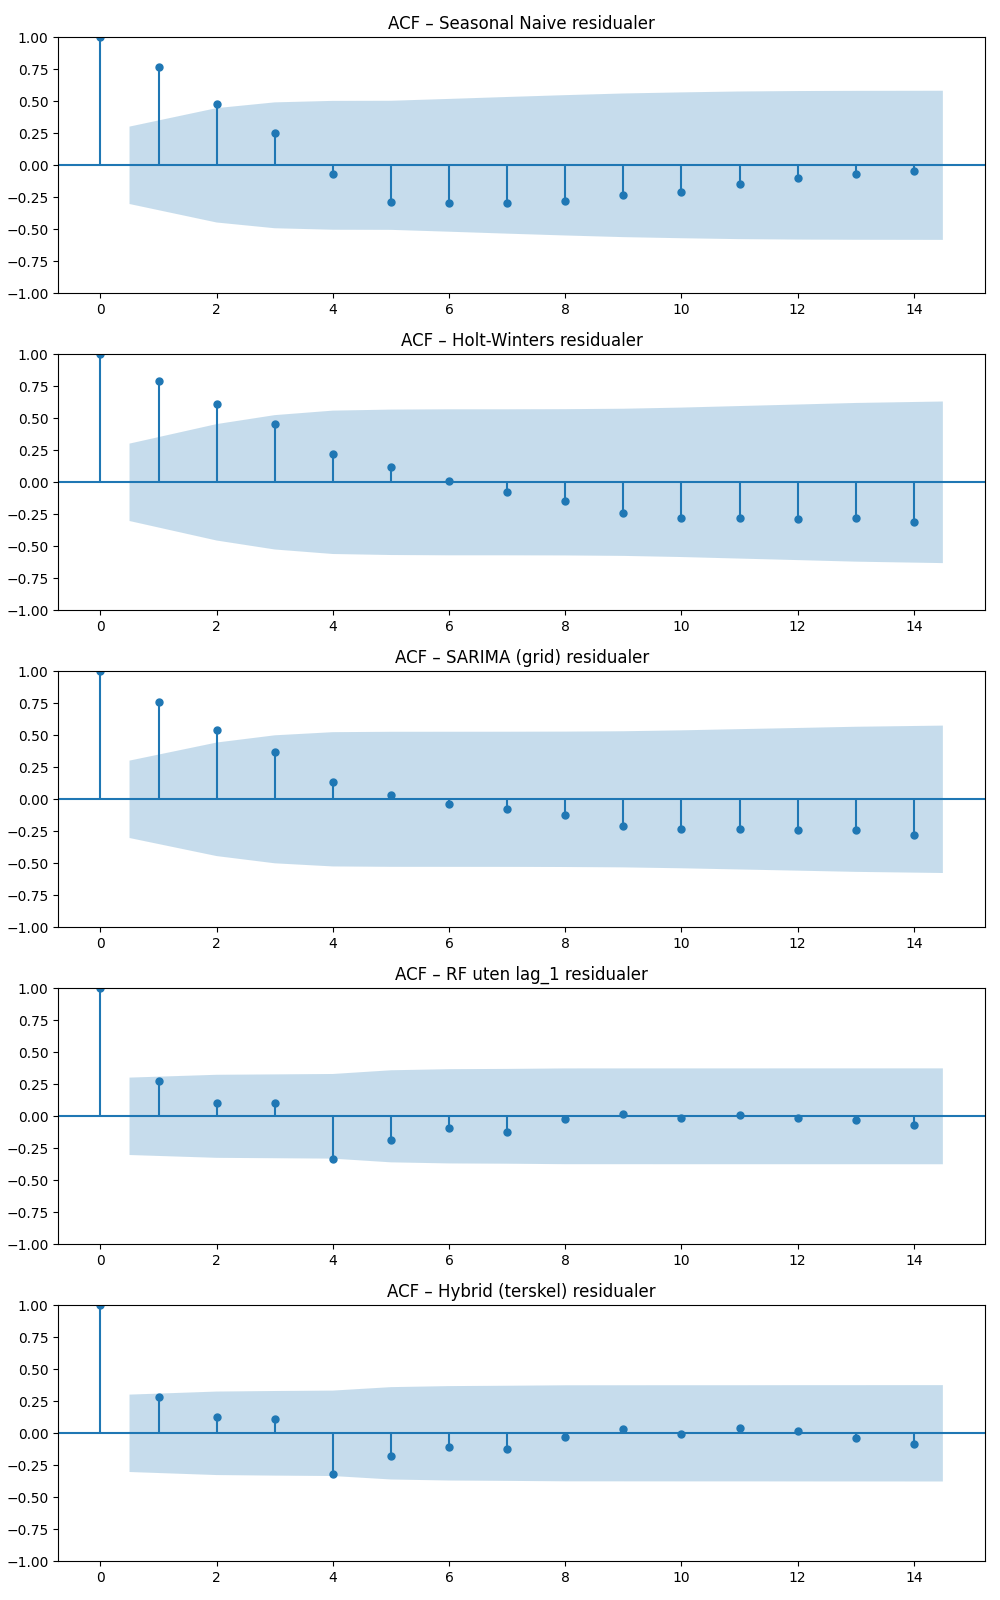
\includegraphics[keepaspectratio,alt={Figur 6: ACF-plott av residualene}]{figurer/fig6_residual_acf.png}}
\caption{Figur 6: ACF-plott av residualene}
\end{figure}

\emph{Figur 6: ACF-plott av residualene for fem sentrale modeller
(Seasonal Naive, Holt-Winters, SARIMA, RF uten lag\_1 og Hybrid
terskel). Blått felt indikerer konfidensintervall for hvit støy;
residualer som holder seg innenfor feltet betyr at modellen har
ekstrahert all systematisk informasjon.}

Tabell 7 og Figur 6 viser et markant skille: tidsseriemodellene (Naive,
HW, SARIMA) og GBM har signifikant autokorrelasjon i residualene, det
vil si at de ikke har fanget opp all struktur. Random Forest, RF uten
lag\_1 og hybridene har residualer som er statistisk uavhengige, og har
dermed ekstrahert den systematiske informasjonen fra datasettet.
Diagnostisk implikasjon for modellvalg drøftes i kap. 9.3.

Oppsummert viser resultatene at modellene tilbyr \emph{komplementære
styrker}: SARIMA gir best presisjon i normaldrift, RF uten lag\_1 gir
best ytelse på kampanje- og toppdager, og hybridene kombinerer styrkene
med balanserte bias. Dette gir grunnlag for en nyansert diskusjon i kap.
9.

\section{9. Diskusjon}\label{diskusjon}

Dette kapittelet drøfter funnene fra analysen og vurderer de
operasjonelle konsekvensene for REMA 1000 Distribusjon Trondheim.
Kapittelet er strukturert rundt seks temaer: (9.1) datakvalitet og
metodiske erfaringer, (9.2) verdien av informasjonsdeling (Scenario 1 vs
2), (9.3) modellenes komplementære roller, (9.4) hybridenes
routing-utfordring, (9.5) praktiske implikasjoner, og (9.6) metodiske
begrensninger.

\subsection{9.1 Datakvalitet og metodisk
erfaring}\label{datakvalitet-og-metodisk-erfaring}

En viktig metodisk erfaring i prosjektet var oppdagelsen av en datafeil
i det opprinnelige vaskeskriptet. Første iterasjon av analysen brukte en
aggregert tidsserie med sum 6 201 stk, mens faktisk
\texttt{Bestilt\ antall} i råfilen summerer til 20 934 stk, en
undertelling på \textasciitilde70 \%. Feilen ble oppdaget ved kryssjekk
mot en uavhengig RELEX-eksport (20 801 stk), og skyldtes sannsynligvis
en utdatert versjon av den vaskede filen som ikke ble regenerert etter
at råfilen ble oppdatert. Vaskeskriptet selv produserer korrekte tall
når det kjøres på dagens rådata.

Denne erfaringen understøtter et metodisk hovedpoeng: kryssjekk mot
uavhengige datakilder er essensielt i prognosearbeid. Totalsummer og
dagsgjennomsnitt bør valideres tidlig i prosessen, ikke tolkes som gitt.
Resultatene i rapporten bygger på den verifiserte RELEX-eksporten, som
krysstemmer innen 0,6 \% mot ERP-uttrekket på transaksjonsnivå (jf. kap.
4.3, datakildekontrolltabell).

Oppdagelsen førte også til andre metodiske justeringer: - Overgang fra
7-dagers til 5-dagers sesongsyklus (virkedager), siden RD Trondheim ikke
ekspederer i helg. - Innføring av robuste evalueringsmål (sMAPE, WAPE)
som supplerer MAPE. MAPE er nærmest ubrukelig på lavt volum (verdier opp
mot 2 973 \% på enkelte segmenter), slik Hyndman og Koehler (2006)
påpeker. - Formell residualdiagnostikk med Ljung-Box-test som supplement
til visuell ACF-inspeksjon.

\subsection{9.2 Verdien av informasjonsdeling (Scenario 1 vs
2)}\label{verdien-av-informasjonsdeling-scenario-1-vs-2}

Sammenligningen mellom Scenario 1 (blind) og Scenario 2 (med
kampanjeinfo) viser en nyansert effekt av informasjonsdeling. Effekten
varierer kraftig mellom modeller og segmenter:

\begin{itemize}
\tightlist
\item
  \textbf{SARIMA på normale dager:} stor forbedring, MAE reduseres fra
  46,0 (S1) til 29,4 (S2), en nedgang på 36 \%. Kampanjeflagget gir
  SARIMA et signal om å suspendere ren historisk inferens på markerte
  dager, slik at sesongmønsteret de øvrige dagene blir tydeligere.
\item
  \textbf{RF uten lag\_1 totalt:} moderat forbedring, MAE 179 → 169 (5,5
  \% bedre).
\item
  \textbf{Random Forest, Gradient Boosting totalt:} \emph{dårligere} med
  kampanjeinfo. Scenario 2 øker RF-feilen fra 183 til 192, og GBM fra
  268 til 294.
\item
  \textbf{SARIMA på toppdager:} \emph{dårligere} med kampanjeinfo (MAE
  405 → 432). Binært kampanjeflagg er for grovt, ettersom modellen lærer
  at ``kampanje = høy'', men responsen på Crazy Days vs jul vs påske
  varierer dramatisk.
\end{itemize}

Resultatene understøtter Trapero et al.~(2015)s generelle poeng om at
kampanjekalender-integrasjon reduserer systematiske feil, men legger til
et nyanserende funn: binære kampanjeindikatorer er ikke nok. For å
realisere gevinstene fullt ut trenger modellene rikere
kampanjerepresentasjon, for eksempel forventet volum eller priseffekter.
Dette er en konkret anbefaling for videre arbeid.

Mekanismen bak svikten er konsistent på tvers av modellfamilier: et
binært flagg lar modellene lære at «kampanje = høy», men koder ikke
magnituden eller karakteren av kampanjen. På Crazy Days vinter (uke
5/2026) når dagsvolumet over 1 300 stk, mens på en mindre hendelsesdag
(f.eks. mandag etter nyttår) ligger volumet på 200--400 stk. Med samme
flaggverdi (1) for begge tilfeller ender modellen opp med å predikere et
middelnivå som blir for lavt for Crazy Days og for høyt for mindre
kampanjer, og denne over-aggregerte signalrepresentasjonen er en
hovedmekanisme bak de store residualene observert på toppdager (jf.
Tabell 6 i kap. 8.3 og Figur 5). Det er nettopp den uniforme kodingen
som motiverer anbefalingen om rikere kampanjedata: differensierte
signaler om forventet volum eller priseffekt ville gitt modellene
mulighet til å skille mellom kampanjetypene og dermed dempe
topp-spesifikke feil.

\subsection{9.3 Modellenes komplementære
roller}\label{modellenes-komplementuxe6re-roller}

Analysen viser at det ikke finnes én beste modell, og at ulike modeller
vinner på ulike segmenter:

\begin{itemize}
\tightlist
\item
  \textbf{SARIMA (grid)} er best i normaldrift (MAE 29,4 på normale
  dager). Den fanger ukedagssyklusen og rutinemessig sesongvariasjon
  presist.
\item
  \textbf{RF uten lag\_1} er best på toppdager (MAE 290,2). Når
  \texttt{lag\_1} utelates, tvinges modellen til å bruke bredere
  sesongkontekst (\texttt{rolling\_mean\_5}, \texttt{lag\_5},
  \texttt{lag\_10}), som gjør den robust mot ekstreme utslag.
\item
  Den opprinnelige Random Forest med lag\_1 har feature
  importance-dominans (lag\_1 = 84 \%, jf. vedlegg A4) og fungerer i
  praksis som en forsterket ``i morgen = i dag''-modell. Dette forklarer
  både hvorfor den har uavhengige residualer (lag\_1 fanger
  autoregressiv struktur) og hvorfor den feiler på toppdager (lag\_1 er
  ikke-informativ når etterspørselen plutselig hopper).
\end{itemize}

En strukturell asymmetri forklarer hvorfor tidsseriemodellene
systematisk ikke når toppdagenes nivå: klassisk sesongutjevning glatter
mot et historisk gjennomsnitt og kan dermed ikke produsere de ekstreme
verdiene kampanjedrift krever. Dette manifesterer seg konkret i kap.
8.3, der både Holt-Winters og SARIMA har \textbar Bias\textbar{} ≈ MAE
på toppdager (487 og 432 stk). Når Bias og MAE er like i absoluttverdi
må alle residualer ha samme fortegn, det vil si at samtlige 15 toppdager
underprognoseres systematisk. RF uten lag\_1 unngår dette mønsteret
fordi den ikke er bundet av en lineær glatting og kan produsere
prediksjoner som faktisk treffer toppene, om enn med høyere varians.

Dette er et sterkt argument for at modellvalg bør styres av segmentet
man prognoserer for. En retail-virksomhet som REMA kan ha stor nytte av
å operere med ulike modeller for rutineprognoser vs kampanjeprognoser,
heller enn å tvinge én modell til å passe begge.

Residualdiagnostikken (Tabell 7) supplerer dette bildet. SARIMA har
lavest MAE på normale dager, men residualene avviser Ljung-Box (Q=53,6,
p\textless0,001), og modellen har altså ikke fanget all struktur. RF
uten lag\_1 har residualer som passerer Ljung-Box (p=0,24), men
dårligere punktprognoser på normale dager. Dette kan tolkes som at
SARIMA er ``optimal parametrisk'' innen sine lineære antagelser, mens RF
uten lag\_1 faktisk ekstraherer mer informasjon fra dataene, men med
høyere prediksjonsvarians.

\subsection{9.4 Hybridenes
routing-utfordring}\label{hybridenes-routing-utfordring}

To hybridvarianter ble testet. Den kampanjebaserte hybriden ruter etter
kampanjeflagget (is\_crazy\_days eller is\_event), mens den
terskelbaserte hybriden ruter etter RF uten lag\_1 sin egen prediksjon
(hvis \textgreater{} 70,6 stk → bruk RF uten lag\_1).

Den kampanjebaserte hybriden feilet på toppdager (MAE 445 mot RF uten
lag\_1 alene på 290). Analysen viste at kampanjedager og toppdager ikke
er samme mengde. I testsettet er det toppdager utenfor kampanjeperioder
(f.eks. mandag etter nyttår), og disse rutes feil til SARIMA. Den
terskelbaserte hybriden korrigerer dette ved å la selve
prediksjonsapparatet avgjøre. Resultatet er MAE 305 på toppdager og
nesten null systematisk bias (+6,6 totalt).

Avveiningen er tap av presisjon på noen normale dager (MAE 104 vs
SARIMAs 29), fordi terskelen gir falske positive routinger der RF selv
overpredikerer. Dette er en klassisk klassifikator-avveining:
terskelbasert routing forbedrer toppdager på bekostning av noen normale
dager.

For operasjonell bruk er den terskelbaserte hybridens balanserte bias
(+6,6) mer attraktiv enn SARIMAs sterke negative bias (−170), fordi
bias-skjevhet har større konsekvens for sikkerhetslagerkostnader enn
tilfeldige avvik (Seiringer et al., 2022).

\subsection{9.5 Praktiske implikasjoner for REMA
1000}\label{praktiske-implikasjoner-for-rema-1000}

Siden butikkenes ordrer for tørrvarer godkjennes med nær 100 \% aksept
av AOF/RELEX-forslaget (kap. 4.1), er prognosens kvalitet direkte
styrende for bestilt volum. De observerte MAE-tallene kan derfor
oversettes direkte til operasjonelle konsekvenser:

I normaldrift, som utgjør 27 av 42 testdager og typisk ca. 90 \% av
dagene i et representativt år, gir SARIMA en MAE på 29 stk. Med median
normalt salg på ca. 20 stk (jf. kap. 4.3) er dette et grovt nivå, men
fortsatt brukbart, og kan reduseres med mer enn halvparten ved presist
modellvalg. På toppdager (15 av 42 testdager, primært kampanjer og
høytider) gir RF uten lag\_1 MAE 290 stk. Med et absoluttvolum på 1
000--2 000 stk innebærer dette en typisk relativ feil på 15--30 \%.
Dette er en kritisk feilmargin som må suppleres med menneskelig skjønn
og nær koordinasjon mellom distribusjonslageret, regionskontor og
kampanjeplanleggerne hos REMA sentralt.

\textbf{Konkret anbefaling:} REMA 1000 bør bruke ulike modeller for
ulike beslutningskontekster: 1. Daglig volumbestilling i normaldrift:
SARIMA med kampanjeflagg. 2. Kampanje- og høytidsplanlegging: RF uten
lag\_1 kombinert med manuelle overstyringer basert på eksplisitt
forventet kampanjemagnitude (ikke bare binært flagg). 3. Månedlig
kapasitetsplanlegging: terskelbasert hybrid som kompromissmodell med
balansert bias.

Dette er i tråd med Fildes et al.~(2009) sin observasjon om at
menneskelige overstyringer basert på unik lokalkunnskap kan forbedre
prognoser, så lenge de anvendes systematisk heller enn ukritisk.

\subsection{9.6 Metodiske begrensninger}\label{metodiske-begrensninger}

Den første begrensningen gjelder testsettets sammensetning.
Januar--februar 2026 inneholder Crazy Days vinter (uke 5) og den
etterfølgende toppuken (uke 6, med dagsverdier opp mot 1 378 stk). Av 42
testdager er 15 (36 \%) klassifisert som toppdager, betydelig over den
forventede andelen på ca. 10 \% i et representativt år. De globale
feilmålene i Tabell 5 er derfor sterkt påvirket av toppdagene, og
sammenligninger mellom modeller på globalt nivå må tolkes med varsomhet.
Den segmenterte analysen i kap. 8.3 er rapportens primære lens for
modellvalg, nettopp fordi den isolerer normaldrift og kampanjedrift.

En andre begrensning er fraværet av walk-forward-validering.
Evalueringen bygger på en enkelt fast trenings-/testsplitt (83/17 \%).
Med kun 42 testdager er resultatene sårbare for tilfeldigheter i hvilke
datoer som faller i testperioden. En walk-forward-validering (expanding
window) ville gitt mer robuste estimater og mulighet til å kvantifisere
prognoseusikkerhet over tid. Dette er et naturlig neste steg for videre
arbeid (se kap. 10).

En tredje vurdering knytter seg til risikoen for overdifferensiering i
SARIMA. ADF-testen (kap. 7.1, Tabell A1) indikerer at treningsserien
allerede er stasjonær (p \textless{} 0,001). Likevel valgte
AIC-minimerende grid-søk en modell med både vanlig og
sesongdifferensiering (\(d=1, D=1\)). Grid-søket inkluderte også
\(d=0, D=0\)-kombinasjoner, så valget er datastyrt, men AIC straffer
ikke overdifferensiering per se. Double differencing på en allerede
stasjonær serie kan introdusere kunstig MA-struktur (MA-koeffisient nær
\(-1\)), noe som delvis kan forklare den systematiske underestimeringen
på toppdager (jf. kap. 8.3 og Hyndman \& Athanasopoulos, 2021). En
parsimonisk \((p,0,q)(P,0,Q)_5\)-modell bør vurderes i et videre arbeid
som sensitivitetssjekk.

En femte begrensning er studiens generaliserbarhet. Funnene gjelder ett
produkt (Lasagne Familiepakning, en kampanjedrevet tørrvare med lavt
normalvolum og kraftige topper) ved ett distribusjonssenter (RD
Trondheim) over én tidsperiode (mars 2025 -- februar 2026). Den
observerte segmentstrukturen, der SARIMA dominerer normaldrift og RF
uten lag\_1 dominerer toppdager, er sannsynligvis robust for andre
kampanjedrevne tørrvarer i samme distribusjonsnettverk fordi den
underliggende mekanismen (ukedags-sesong med kraftige men sjeldne
toppspisser) er felles for kategorien. For ferskvarer med kort
holdbarhet er etterspørselssignalet typisk mindre kampanjedrevet og mer
knyttet til daglige forbruksmønstre, slik at modellrangeringen kan se
annerledes ut. For produkter med jevnere etterspørsel uten
lumpy-komponent vil den segmenterte tilnærmingen miste mye av sin verdi,
ettersom «normaldrift» og «toppdag» ikke utgjør distinkte regimer.
Reproduksjon på flere produkter og tidsperioder er derfor nødvendig før
de praktiske anbefalingene i kap. 9.5 kan løftes til generelle
retningslinjer for hele REMA 1000s sortiment.

En sjette betraktning er en forkastet leveranse: en utvidet
kampanjekalender. I prosjektets løp vurderte vi å utvikle en mer
detaljert kampanjekalenderfil som leveranse, med forventet volum,
varighet per dag og prismetadata, slik at den kunne brukes som rik
eksogen input i modellene. Vi forkastet dette fordi det tilgjengelige
datagrunnlaget kun dekker 12 måneder med to Crazy Days-sykluser og tre
kalenderhendelser. Det gir for få observasjoner til å kalibrere
parametre per kampanjetype, og en slik fil ville i praksis vært dominert
av subjektive antagelser fremfor empirisk grunnlag. Vi anbefaler likevel
generelt at en strukturert, levende kampanjekalender med flerårig
historikk og rikere kampanjemetadata (forventet volum, varighet,
priskontekst) bygges opp som operativ artefakt i prognosearbeid med
kampanjedrevet etterspørsel, slik at den statistiske informasjonen
akkumulerer over tid og kan tas i bruk når datagrunnlaget tillater
meningsfull parametrisering.

Disse begrensningene danner grunnlaget for anbefalingene om videre
arbeid i kap. 10.

\section{10. Konklusjon}\label{konklusjon}

Dette prosjektet har undersøkt hovedproblemstillingen om
prognosepresisjon for ``Lasagne Familiepakning'' ved REMA 1000
Distribusjon Trondheim, strukturert i tre delproblemer: hvordan de
historiske etterspørselsmønstrene kan karakteriseres (delproblem 1),
hvilke modeller gir lavest feilrate (delproblem 2), og i hvilken grad
kampanjeaktivitet begrenser modellenes presisjon (delproblem 3). Åtte
modeller er estimert i to scenarier på et verifisert datagrunnlag på 260
virkedager (218 trening / 42 test).

Hovedkonklusjonene er:

\begin{enumerate}
\def\labelenumi{\arabic{enumi}.}
\item
  \textbf{Etterspørselsmønsteret er kampanjedrevet med lavt normalvolum
  (delproblem 1).} Daglig utlevert volum kjennetegnes av lavt
  normalvolum (treningssettets median 19,5 stk og gjennomsnitt 61,1
  stk), høy spredning (standardavvik 239,3 stk), tydelig virkedagseffekt
  (sterke ACF-topper ved lag 5, 10 og 15, jf. kap. 7.1), og kraftige
  kampanjetopper med dagsverdier opp mot 2 172 stk i treningssettet.
  Mønsteret faller i Syntetos og Boylan (2005) sin kategori for «lumpy
  demand» og motiverer både segmentert evaluering (normale dager vs
  toppdager) og parallell bruk av tidsserie- og maskinlæringsbaserte
  modeller.
\item
  \textbf{Modellvinnerne er segmentspesifikke (delproblem 2).} SARIMA
  med grid-søkt parametervalg og eksogene kampanjevariabler har lavest
  MAE i normaldrift (29,4 stk). Random Forest uten lag\_1 har lavest MAE
  på toppdager (290,2 stk). Ingen enkeltmodell dominerer begge
  segmenter, og valg av modell bør tilpasses den operative
  beslutningskonteksten (jf. anbefaling i kap. 9.5).
\item
  \textbf{Informasjonsdeling har begrenset og ujevn effekt (delproblem
  3).} Tillegg av binær kampanjeinfo (Scenario 2) gir tydelig gevinst
  kun på SARIMA i normaldrift (−36 \% MAE). På toppdager gir
  kampanjeflagg marginal eller negativ gevinst for fem av seks modeller
  (alle unntatt RF uten lag\_1). Binær kampanjerepresentasjon er for
  grov til å fange den faktiske varians i kampanjerespons. For å
  realisere full verdi av informasjonsdeling anbefales rikere
  kampanjedata (forventet volum, priseffekter).
\item
  \textbf{Hybridmodeller viser potensiale men krever presis routing.} En
  kampanjebasert routing feilet fordi kampanjedager og toppdager ikke er
  samme mengde. En terskelbasert routing (baserer rutingen på RF uten
  lag\_1 sin egen prediksjon) leverer balansert ytelse med nesten null
  global bias (+6,6 stk), og er operasjonelt attraktiv for
  sikkerhetslagerdimensjonering.
\item
  \textbf{Residualdiagnostikk differensierer modellvaliditeten.}
  Ljung-Box-test (10 etterslep / lags) avslører at tidsseriemodellene
  (Naive, Holt-Winters, SARIMA) og GBM har signifikant autokorrelasjon i
  residualene, og at de ikke har fanget all systematisk struktur. RF, RF
  uten lag\_1 og hybridene har residualer som passerer testen, og
  ekstraherer dermed informasjonen fullstendig. Dette er et sterkt
  argument for de tre-baserte modellenes validitet, selv når de ikke har
  lavest MAE.
\item
  \textbf{Metodisk lærdom (jf. kap. 9.1):} Datafeilen oppdaget tidlig i
  prosjektet understreker behovet for systematisk kryssjekk mot
  uavhengige datakilder, og at metodisk infrastruktur (grid-search,
  kryssvalidert tuning, formelle residualtester) bør være på plass fra
  starten av analysen.
\end{enumerate}

Samlet viser prosjektet at en parallell bruk av tidsserie- og
maskinlæringsbaserte modeller gir akseptabel presisjon for dette
produktet ved RD Trondheim, men at kampanjer og høytider krever både
rikere eksogen informasjon og segmentbaserte modellvalg. Når butikkenes
ordrer godkjennes med nær 100 \% aksept av AOF/RELEX-forslag (kap. 4.1),
får prognosekvaliteten direkte operativ betydning for bestilte volum,
lagerbinding og leveringssikkerhet.

Videre arbeid bør prioritere tre områder. For det første anbefales
integrasjon av forventet kampanjevolum fra REMA sentralt / regionskontor
i prognosemodellene, eventuelt formalisert som en strukturert, flerårig
kampanjekalender med forventet volum, varighet og priskontekst per
kampanje (jf. kap. 9.6). For det andre vil walk-forward-validering gi
mer robust evaluering. For det tredje anbefales ekspansjon til flere
produktkategorier, særlig ferskvarer der kort holdbarhet gjør at
overprognose direkte oversettes til svinn.

\newpage

\section{11. Bibliografi}\label{bibliografi}

Arunraj, N. S., \& Ahrens, D. (2015). A hybrid seasonal autoregressive
integrated moving average and quantile regression for daily food sales
forecasting. \emph{International Journal of Production Economics}, 170,
147-160. https://doi.org/10.1016/j.ijpe.2015.09.014

Box, G. E. P., \& Jenkins, G. M. (1976). \emph{Time series analysis:
Forecasting and control} (rev. utg.). Holden-Day.

Breiman, L. (2001). Random forests. \emph{Machine Learning}, 45(1),
5-32. https://doi.org/10.1023/A:1010933404324

Dickey, D. A., \& Fuller, W. A. (1979). Distribution of the estimators
for autoregressive time series with a unit root. \emph{Journal of the
American Statistical Association}, 74(366a), 427-431.
https://doi.org/10.1080/01621459.1979.10482531

Fildes, R., Goodwin, P., Lawrence, M., \& Nikolopoulos, K. (2009).
Effective forecasting and judgmental adjustments: an empirical
evaluation and strategies for improvement in supply-chain planning.
\emph{International Journal of Forecasting}, 25(1), 3-23.
https://doi.org/10.1016/j.ijforecast.2008.11.010

Fildes, R., Ma, S., \& Kolassa, S. (2022). Retail forecasting: Research
and practice. \emph{International Journal of Forecasting}, 38(4),
1269-1295. https://doi.org/10.1016/j.ijforecast.2021.11.004

Friedman, J. H. (2001). Greedy function approximation: A gradient
boosting machine. \emph{Annals of Statistics}, 29(5), 1189-1232.
https://doi.org/10.1214/aos/1013203451

Hyndman, R. J., \& Athanasopoulos, G. (2021). \emph{Forecasting:
Principles and practice} (3. utg.). OTexts. https://otexts.com/fpp3/

Hyndman, R. J., \& Koehler, A. B. (2006). Another look at measures of
forecast accuracy. \emph{International Journal of Forecasting}, 22(4),
679-688. https://doi.org/10.1016/j.ijforecast.2006.03.001

Ljung, G. M., \& Box, G. E. P. (1978). On a measure of lack of fit in
time series models. \emph{Biometrika}, 65(2), 297-303.
https://doi.org/10.1093/biomet/65.2.297

Makridakis, S., Spiliotis, E., \& Assimakopoulos, V. (2022). The M5
competition: Background, organization, and results. \emph{International
Journal of Forecasting}, 38(4), 1325-1346.
https://doi.org/10.1016/j.ijforecast.2021.01.005

Seiringer, W., Brockmann, F., Altendorfer, K., \& Felberbauer, T.
(2022). Influence of forecast error and forecast bias on safety stock on
a MRP system with rolling horizon forecast updates. I \emph{Operations
Research Proceedings 2021} (kap. 62). Springer.
https://doi.org/10.1007/978-3-031-08623-6\_62

Syntetos, A. A., \& Boylan, J. E. (2005). The accuracy of intermittent
demand estimates. \emph{International Journal of Forecasting}, 21(2),
303-314. https://doi.org/10.1016/j.ijforecast.2004.10.001

Syntetos, A. A., Boylan, J. E., \& Disney, S. M. (2009). Forecasting for
inventory planning: a review. \emph{Journal of the Operational Research
Society}, 60(1), S149-S160. https://doi.org/10.1057/jors.2008.173

Trapero, J. R., Kourentzes, N., \& Fildes, R. (2015). On the importance
of forecasting promotional sales: A retail case study.
\emph{International Journal of Forecasting}, 31(4), 1166-1176.
https://doi.org/10.1016/j.ijforecast.2015.06.001

\subsubsection{Programvare og
biblioteker}\label{programvare-og-biblioteker}

McKinney, W. (2010). Data structures for statistical computing in
Python. \emph{Proceedings of the 9th Python in Science Conference},
51-56. https://doi.org/10.25080/Majora-92bf1922-00a

Pedregosa, F., Varoquaux, G., Gramfort, A., Michel, V., Thirion, B.,
Grisel, O., Blondel, M., Prettenhofer, P., Weiss, R., Dubourg, V.,
Vanderplas, J., Passos, A., Cournapeau, D., Brucher, M., Perrot, M., \&
Duchesnay, É. (2011). Scikit-learn: Machine learning in Python.
\emph{Journal of Machine Learning Research}, 12, 2825-2830.

Seabold, S., \& Perktold, J. (2010). Statsmodels: Econometric and
statistical modeling with Python. \emph{Proceedings of the 9th Python in
Science Conference}, 92-96. https://doi.org/10.25080/Majora-92bf1922-011

\newpage

\section{12. Vedlegg}\label{vedlegg}

\subsection{A1 --- ADF-test for stasjonaritet i
treningsserien}\label{a1-adf-test-for-stasjonaritet-i-treningsserien}

Augmented Dickey-Fuller-test (H0: enhetsrot, ikke-stasjonær). p
\textless{} 0,05 → avvises.

{\def\LTcaptype{none} % do not increment counter
\begin{longtable}[]{@{}lrrrl@{}}
\toprule\noalign{}
Serie & ADF-stat & p-verdi & Kritisk (5 \%) & Stasjonær? \\
\midrule\noalign{}
\endhead
\bottomrule\noalign{}
\endlastfoot
Rå (faktisk\_ettersporsel) & −5,01 & \textless{} 0,001 & −2,88 & Ja \\
1. ordens differensiert & −8,17 & \textless{} 0,001 & −2,88 & Ja \\
Sesongdifferensiert (s=5) & −5,36 & \textless{} 0,001 & −2,88 & Ja \\
\end{longtable}
}

Kilde: \texttt{004\ data/adf\_test.csv}. Serien er stasjonær uten
differensiering. AIC-minimerende grid-søk (kap. 7.2) valgte likevel en
modell med både vanlig og sesongdifferensiering (\(d=1, D=1\)); risikoen
for overdifferensiering på en allerede stasjonær serie er drøftet i kap.
9.6.

\subsection{A2 --- SARIMA grid-search (utdrag: topp 5 og valgt
modell)}\label{a2-sarima-grid-search-utdrag-topp-5-og-valgt-modell}

144 kombinasjoner av \((p,d,q)(P,D,Q)_5\) ble estimert på treningssettet
med eksogene regressorer (\texttt{is\_crazy\_days}, \texttt{is\_event}).
Utvalg er minst AIC blant modeller som konvergerte (omtalt i kap. 7.2).

{\def\LTcaptype{none} % do not increment counter
\begin{longtable}[]{@{}rllrrl@{}}
\toprule\noalign{}
Rang & order & seasonal\_order & AIC & BIC & Konvergerte \\
\midrule\noalign{}
\endhead
\bottomrule\noalign{}
\endlastfoot
1 (valgt) & (0,1,2) & (0,1,1)\_5 & 2 510,06 & 2 529,67 & Ja \\
2 & (0,1,2) & (1,1,1)\_5 & 2 511,96 & 2 534,83 & Ja \\
3 & (1,1,2) & (1,1,1)\_5 & 2 533,97 & 2 560,12 & Ja \\
4 & (1,0,2) & (0,0,1)\_5 & 2 537,94 & 2 561,02 & Ja \\
5 & (1,0,2) & (1,1,0)\_5 & 2 551,51 & 2 574,49 & Ja \\
\end{longtable}
}

Fullstendig grid i \texttt{004\ data/sarima\_diagnostikk.csv}.
Forbedring mot original konfigurasjon \((1,1,1)(1,1,1)_7\) (AIC 2 558):
48 AIC-poeng. Merk: Flere ordner med numerisk lavere AIC (helt ned mot 2
481, jf. kap. 7.2) hadde konvergensproblemer og ble derfor ikke valgt.
AIC-verdiene over er vist med to desimaler for presisjon; hovedteksten i
kap. 7.2 bruker avrundede verdier (2 510, 2 558, 2 481) for lesbarhet.

\subsection{A3 --- Gradient Boosting
hyperparameter-tuning}\label{a3-gradient-boosting-hyperparameter-tuning}

3-fold TimeSeriesSplit-kryssvalidering,
scoring=neg\_mean\_absolute\_error. 16 kombinasjoner.

\textbf{Valgt hyperparametersett:} - \texttt{learning\_rate} = 0,05 -
\texttt{max\_depth} = 2 - \texttt{n\_estimators} = 100 -
\texttt{subsample} = 1,0

Fullstendig grid i \texttt{004\ data/gbm\_tuning.csv}. Tunet GBM gir
\textasciitilde30 \% bedre MAE enn utunet standard (Sklearn-defaults:
\texttt{learning\_rate=0,1}, \texttt{max\_depth=3},
\texttt{n\_estimators=100}, jf. kap. 7.2).

\subsection{A4 --- Feature importance i Random
Forest-modellene}\label{a4-feature-importance-i-random-forest-modellene}

Tabellen oppsummerer feature importance for de tre tre-baserte
modellene; lag\_1-dominansen i full RF-variant (84 \%) og
redistribusjonen i RF uten lag\_1-varianten er omtalt i kap. 7.2 og kap.
9.3.

{\def\LTcaptype{none} % do not increment counter
\begin{longtable}[]{@{}lrrr@{}}
\toprule\noalign{}
Feature & RF (full) & GBM & RF uten lag\_1 \\
\midrule\noalign{}
\endhead
\bottomrule\noalign{}
\endlastfoot
lag\_1 & 0,840 & 0,791 & -- \\
rolling\_mean\_5 & 0,074 & 0,128 & 0,459 \\
lag\_5 & 0,018 & 0,031 & 0,253 \\
lag\_10 & 0,023 & 0,002 & 0,144 \\
week\_of\_month & 0,013 & 0,000 & 0,056 \\
is\_monday & 0,008 & 0,000 & 0,004 \\
month & 0,004 & 0,000 & 0,020 \\
Øvrige (dag-dummier, kampanjeflagg) & 0,020 & 0,048 & 0,064 \\
\end{longtable}
}

Fullstendig tabell i \texttt{004\ data/rf\_feature\_importance.csv}.

\subsection{A5 --- Random
Forest-hyperparametere}\label{a5-random-forest-hyperparametere}

{\def\LTcaptype{none} % do not increment counter
\begin{longtable}[]{@{}ll@{}}
\toprule\noalign{}
Parameter & Verdi \\
\midrule\noalign{}
\endhead
\bottomrule\noalign{}
\endlastfoot
\texttt{n\_estimators} & 100 \\
\texttt{random\_state} & 42 \\
\texttt{max\_depth} & None (ingen grense) \\
\texttt{min\_samples\_split} & 2 (default) \\
\texttt{min\_samples\_leaf} & 1 (default) \\
\texttt{max\_features} & 1.0 (default for regresjon) \\
\end{longtable}
}

\texttt{random\_state=42} sikrer reproduserbarhet av tilfeldig utvalg i
bootstrap og feature subsampling, slik at modellen gir identiske
resultater ved gjentatte kjøringer.

\subsection{A6 --- Kampanjekalender}\label{a6-kampanjekalender}

Lagret i \texttt{004\ data/kampanjekalender.csv}, lest inn ved
modellkjøring.

{\def\LTcaptype{none} % do not increment counter
\begin{longtable}[]{@{}
  >{\raggedright\arraybackslash}p{(\linewidth - 8\tabcolsep) * \real{0.2000}}
  >{\raggedright\arraybackslash}p{(\linewidth - 8\tabcolsep) * \real{0.2000}}
  >{\raggedright\arraybackslash}p{(\linewidth - 8\tabcolsep) * \real{0.2000}}
  >{\raggedright\arraybackslash}p{(\linewidth - 8\tabcolsep) * \real{0.2000}}
  >{\raggedright\arraybackslash}p{(\linewidth - 8\tabcolsep) * \real{0.2000}}@{}}
\toprule\noalign{}
\begin{minipage}[b]{\linewidth}\raggedright
Startdato
\end{minipage} & \begin{minipage}[b]{\linewidth}\raggedright
Sluttdato
\end{minipage} & \begin{minipage}[b]{\linewidth}\raggedright
Type
\end{minipage} & \begin{minipage}[b]{\linewidth}\raggedright
Beskrivelse
\end{minipage} & \begin{minipage}[b]{\linewidth}\raggedright
Kilde
\end{minipage} \\
\midrule\noalign{}
\endhead
\bottomrule\noalign{}
\endlastfoot
2025-04-14 & 2025-04-20 & event & Påskeuke & Kalender (uke 16, 2025) \\
2025-08-11 & 2025-08-17 & event & Skolestart & Kalender (uke 33,
2025) \\
2025-11-03 & 2025-11-09 & crazy\_days & Crazy Days høst & REMA e-post
(uke 45, 2025) \\
2025-12-15 & 2025-12-21 & event & Jul & Kalender (uke 51, 2025) \\
2026-01-26 & 2026-02-01 & crazy\_days & Crazy Days vinter & REMA e-post
(uke 5, 2026) \\
\end{longtable}
}

\subsection{A7 --- Filstruktur og
reproduserbarhet}\label{a7-filstruktur-og-reproduserbarhet}

Analysekoden og datafiler ligger i følgende mappestruktur i prosjektets
Git-repo:

\begin{verbatim}
G27-workin/
├── 004 data/
│   ├── vasket_salg_daglig.csv            — renset daglig etterspørsel (260 virkedager)
│   ├── kampanjekalender.csv               — kampanjer og hendelser
│   ├── sarima_diagnostikk.csv             — grid-search resultater (A2)
│   ├── gbm_tuning.csv                     — hyperparameter-søk (A3)
│   ├── rf_feature_importance.csv          — feature importance (A4)
│   ├── adf_test.csv                       — stasjonaritetstest (A1)
│   ├── residual_diagnostikk.csv           — Ljung-Box-test (Tabell 7)
│   ├── modell_sammendrag.csv              — segmenterte feilmål
│   ├── scenario_sammendrag.csv            — Scenario 1 vs 2, alle modeller og segmenter (kilde for Tabell 4, 5, 6 og 6b)
│   ├── analyse_resultater_stram.csv       — per-dag prediksjoner
│   └── scenario_resultater.csv            — per-dag prediksjoner per scenario
├── 012 fase 2 - plan/
│   ├── vask_relex.py       — datavask fra RELEX-eksport
│   ├── metrics.py          — MAE, MAPE, sMAPE, WAPE, Bias
│   ├── modeller.py         — feature engineering, grid-search, tuning, hybrider
│   ├── analyse_hoved.py    — hovedanalyse (8 modeller)
│   └── scenario_analyse.py — Scenario 1 vs 2 (8 modeller)
└── 014 fase 4 - report/figurer/
    ├── fig1_tidsserie.png
    ├── fig2_ukedag.png
    ├── fig3_bestilling_ukedag.png
    ├── fig4_kampanjeoversikt.png
    ├── fig_a8_lagerstatus.png         (RELEX-skjermbilde, Vedlegg A8)
    ├── fig_scenario_sammenligning.png
    └── fig6_residual_acf.png
\end{verbatim}

Alle analysene kan reproduseres ved å kjøre
\texttt{python\ "012\ fase\ 2\ -\ plan/analyse\_hoved.py"} og
\texttt{python\ "012\ fase\ 2\ -\ plan/scenario\_analyse.py"} fra
prosjektroten.

\subsection{A8 --- Lagerstatus fra RELEX (dokumentasjon på at lageret
aldri var
utsolgt)}\label{a8-lagerstatus-fra-relex-dokumentasjon-puxe5-at-lageret-aldri-var-utsolgt}

Skjermbildet nedenfor er hentet fra REMA 1000s RELEX-grensesnitt og
viser lagerstatus, salg og eksisterende prognose for Lasagne
Familiepakning ved RD Trondheim gjennom hele analyseperioden (mars 2025
-- februar 2026). Skjermbildet er brukt som dokumentasjon på at
lagernivået (sort strek) aldri når null. Distribusjonssenteret har
dermed aldri vært utsolgt på denne varen i perioden, og observerte
salgstall kan tolkes som reell utlevert etterspørsel (se kap. 5.3 og
kap. 4.5).

\begin{figure}
\centering
\pandocbounded{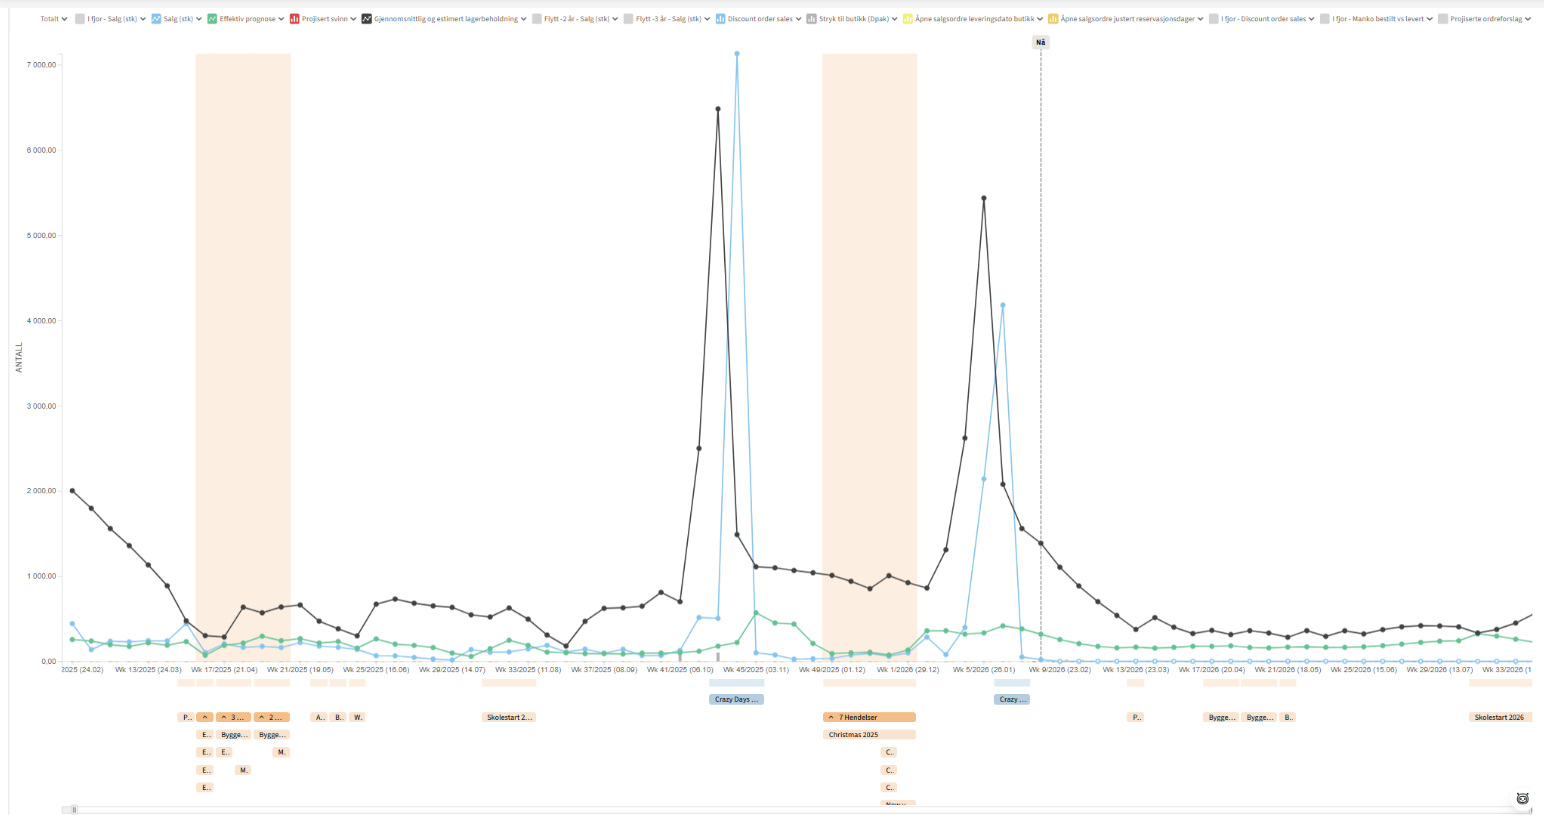
\includegraphics[keepaspectratio,alt={Vedlegg A8: RELEX-skjermbilde av lagerstatus, salg og prognose}]{figurer/fig_a8_lagerstatus.png}}
\caption{Vedlegg A8: RELEX-skjermbilde av lagerstatus, salg og prognose}
\end{figure}

\emph{Vedlegg A8: Skjermbilde fra RELEX-grensesnittet. Varebeholdning
(sort strek), faktisk salg (blå strek) og eksisterende RELEX-prognose
(grønn strek). Markeringer under x-aksen viser kampanjer (blå) og
hendelser (oransje). Kilde: REMA 1000 RELEX-interface, mars 2026.}

\subsection{A9 --- Bruk av KI-verktøy (bruk av kunstig
intelligens)}\label{a9-bruk-av-ki-verktuxf8y-bruk-av-kunstig-intelligens}

Dette vedlegget oppfyller kravet om å dokumentere bruk av kunstig
intelligens (KI) på hjemmeeksamen ved Høgskolen i Molde, i tråd med
KI-retningslinjene og skjemaet «Erklæring om bruk av kunstig intelligens
(KI) på hjemmeeksamen».

\subsubsection{Erklæring}\label{erkluxe6ring}

Har du benyttet KI-verktøy i din besvarelse? {[}x{]} JA {[} {]} NEI

Til hvilke formål KI-verktøyet er brukt:

\begin{itemize}
\tightlist
\item[$\boxtimes$]
  Generere tekst / skrivehjelp
\item[$\boxtimes$]
  Språkvask og korrekturlesing
\item[$\boxtimes$]
  Programmering og kodehjelp
\item[$\boxtimes$]
  Hjelp til å analysere digitale data
\item[$\square$]
  Lage bilder og figurer
\item[$\boxtimes$]
  Annet (strukturering av rapporten og intern kvalitetssikring)
\end{itemize}

Vi bekrefter at en detaljert forklaring av hvilke KI-verktøy som er
brukt, og hvordan de er brukt, er gitt nedenfor. Vi er kjent med
retningslinjene for bruk av KI på hjemmeeksamen ved Høgskolen i Molde,
og teksten som er levert inn er vår egen, uavhengig av KI-verktøy.

Line Lyngsnes Johansen og Amanda Arnesen Almaas, Trondheim, 31. mai
2026.

\subsubsection{Detaljert forklaring}\label{detaljert-forklaring}

Verktøyene som er brukt er Claude (Anthropic, benyttet via Claude Code),
Gemini (Google) og ChatGPT (OpenAI). KI er anvendt som et støtteverktøy
gjennom hele prosjektet, på følgende måter:

\begin{itemize}
\tightlist
\item
  Programmering og kodehjelp: utvikling og feilsøking av
  Python-skriptene for datavask, modellering og scenarioanalyse (blant
  annet \texttt{vask\_relex.py}, \texttt{modeller.py},
  \texttt{analyse\_hoved.py} og \texttt{scenario\_analyse.py}).
\item
  Hjelp til å analysere digitale data: forklaring av statistiske og
  metodiske begreper, drøfting av modellvalg, og tolkning av diagnostikk
  (ADF-test, ACF/PACF og Ljung-Box). Selve beregningene er utført av vår
  egen kode.
\item
  Skrivehjelp og språkvask: utkast, omskriving, korrekturlesing og
  konsistenssjekk av rapporttekst.
\item
  Strukturering og kvalitetssikring: forslag til kapittelstruktur og
  oppbygning, samt intern gjennomgang av tekst, tabeller og figurer.
\end{itemize}

KI er ikke brukt til å generere data, resultater eller kilder. Alt
datagrunnlag stammer fra REMA 1000 (RELEX- og ERP-uttrekk), alle
modellresultater er produsert av vår egen kode, og figurene er laget med
vår egen matplotlib-kode og er ikke KI-genererte bilder. Alle kilder i
bibliografien er funnet, lest og verifisert av oss.

Vurdering og revisjon av KI-forslag: Vi har behandlet KI-genererte
forslag som utkast og innspill, ikke som ferdige svar. Kodeforslag ble
kjørt, testet og rettet mot faktiske data før de ble tatt i bruk, og
tekstforslag ble omskrevet til vårt eget språk og kontrollert mot pensum
og kilder. Faktapåstander og litteraturhenvisninger ble verifisert mot
primærkildene; et konkret eksempel er korrigeringen av publiseringsåret
for Seiringer et al.~(fra 2024 til 2022) etter at vi kontrollerte DOI
mot forlaget.

Refleksjon over påvirkning på tankeprosess og resultat: Bruken av KI
gjorde arbeidet mer effektivt, særlig i koding og i bearbeiding av
tekst, og verktøyene fungerte som en faglig sparringspartner som hjalp
oss å stille bedre spørsmål til egne metodevalg. Samtidig erfarte vi at
kritisk kontroll var avgjørende. Den viktigste innsikten i prosjektet,
oppdagelsen av en undertelling i det opprinnelige datagrunnlaget, kom
nettopp fordi vi krysssjekket tall mot uavhengige kilder og ikke stolte
blindt på automatisk genererte resultater. KI påvirket dermed
framdriften og formen på rapporten, men de faglige beslutningene,
tolkningene og konklusjonene er våre egne. Vi står selv ansvarlige for
det faglige innholdet i oppgaven.

\end{document}
